\documentclass[sigplan,review,anonymous]{acmart}\settopmatter{printfolios=true,printccs=false,printacmref=false}

\usepackage{xcolor}
\usepackage{amssymb} 
\usepackage{tikz}
\usepackage[autostyle]{csquotes}
\usepackage{listings}
\usepackage{multirow}
\synctex=1

\usetikzlibrary{positioning}
\usetikzlibrary{arrows,automata}

\title{Handling String-Number Conversion in String Constraint Solving}
\author{}


%%%%%%%%%%%%%%%%%%%%%%%%%%%%%%%%%%%%%%%%%%%%%%%%%%%%%%%%%%%%%%%%%%%%%%%%%%%%%%
\begin{document}
%%%%%%%%%%%%%%%%%%%%%%%%%%%%%%%%%%%%%%%%%%%%%%%%%%%%%%%%%%%%%%%%%%%%%%%%%%%%%%
\newcommand{\hide}[1]{}

\newcommand{\nat}{\mathbb{N}}
\newcommand{\todo}[1]{{\color{blue}TODO: #1}}
\newcommand{\lh}[1]{{\color{orange}Lukas: #1}}
\newcommand{\sti}[1]{\mbox{\textsf{toInt}($#1$)}}
\newcommand{\its}[1]{\mbox{\textsf{toStr}($#1$)}}
\newcommand{\varn}{\mbox{$\mathbb{V}_{\mathbb{Z}}$}}
\newcommand{\vars}{\mbox{$\mathbb{V}_{\Sigma^*}$}}
\newcommand{\cvars}{\mbox{$\mathbb{V}_{\Sigma_\epsilon}$}}
\newcommand{\pvars}{\mbox{$\mathbb{V}_{\sharp}$}}
%\newcommand{\cvar}{\mbox{$V_{\Sigma_\epsilon}$}}
%\newcommand{\cvarone}{\mbox{$V_{\Sigma_\epsilon}$}}
%\newcommand{\cvartwo}{\mbox{$V'_{\Sigma_\epsilon}$}}
\newcommand{\cvarone}{V}
\newcommand{\cvartwo}{V'}
\newcommand{\cvar}{V}
\newcommand{\pvar}{V_\#}
\newcommand{\pvarone}{V_\#}
\newcommand{\pvartwo}{V'_\#}
\newcommand{\modelsof}[1]{[\![#1]\!]}
\newcommand{\true}{\mbox{$\mathsf{true}$}}
\newcommand{\false}{\mbox{$\mathsf{false}$}}
\newcommand{\enc}[1]{[\![#1]\!]}
%\newcommand{\parikhof}[1]{\mathit{Parikh}{(#1)}}
\newcommand{\parikhof}[1]{\mathbb{P}{(#1)}}
\newcommand{\parikhwof}[2]{|#1|_{#2}}
%\newcommand{\semof}[1]{||#1||}
\newcommand{\semof}[1]{\modelsof{#1}}
\newcommand{\decode}[1]{\mathit{decode_{#1}}}
\newcommand{\parikhfof}[1]{\Phi_{\parikhof{#1}}}
\newcommand{\pim}{\alpha}
\newcommand{\syncop}{\Cap}
\newcommand{\syncof}[2]{#1 \syncop #2}
\newcommand{\syncfof}[2]{\Psi_{\syncof {#1} {#2}}}
\newcommand{\syncT}{T_\syncop}


\maketitle


\lstdefinelanguage{JavaScript}{
	keywords={typeof, new, true, false, catch, function, return, null, catch, switch, var, if, in, while, do, else, case, break},
	keywordstyle=\color{blue}\bfseries,
	ndkeywords={class, export, boolean, throw, implements, import, this},
	ndkeywordstyle=\color{darkgray}\bfseries,
	identifierstyle=\color{black},
	sensitive=false,
	comment=[l]{//},
	morecomment=[s]{/*}{*/},
	commentstyle=\color{purple}\ttfamily,
	stringstyle=\color{red}\ttfamily,
	morestring=[b]',
	morestring=[b]"
}





%%%%%%%%%%%%%%%%%%%%%%%%%%%%%%%%%%%%%%%%%%%%%%%%%%%%%%%%%%%%%%%%%%%%%%%%%%%%%%
\section{Introduction} \label{section:introduction}
%%%%%%%%%%%%%%%%%%%%%%%%%%%%%%%%%%%%%%%%%%%%%%%%%%%%%%%%%%%%%%%%%%%%%%%%%%%%%%



String constraint solving has received considerable attention in the constraint solving community, with solvers such as CVC4 and Z3 implmenting solvers of ever-increasing sophistication.  Operations such as substring and string length are widely supported, and recent solvers such as Z3-str3 have shown impressive results.  However, these solvers have limited for operations that convert between strings and integers; string length operations are sometimes well supported, but not parsing a string as an integer or turning an integer value into its string form.  When there is support, it is often limited to ground terms, i.e. at least one side of the conversion must be a constant.  Thus, $v = string2int("5")$ or $v = int2string(5)$ are handled but $v_1 = int2string(v_2)$ will fail.

As solvers such Z3 are applied to symbolic execution of programming languages, this is increasingly becoming a severe limitation.  For many languages such as Java, conversion between integers and strings is a niche operation, and much symbolic execution can be done without supporting it; however, this is not true of some scripting languages, of which JavaScript is the most notable.  JavaScript is a key language---it powers most interactive content on the Web, and increasingly server-side code with nodejs---and it has conversions between strings and integers embedded in the core of its semantics.

\begin{verbatim}
function resetArray(arr) {
  for(var i = 0; i < arr.length; i++) {
    arr[i] = 0
  }
}
\end{verbatim}



A casual glance at the above code reveal no use of strings at all, but the semantics of field access is somewhat unusual in JavaScript: all array indices act like strings, and numeric indices are converted to strings.  Any faithful symbolic execution of JavaScript must handle such conversions for even basic array operations to work correctly; consider the following code snippet that uses {\tt{resetArray}}, with the value of {\tt{x}} shown on the right:

\begin{tabular}{l|c}
	{\tt{x = [0, 1, 2, 3, 4, 5]}} & [0, 1, 2, 3, 4, 5] \\
	{\tt{resetArray(x)}} & [0, 0, 0, 0, 0, 0] \\
	{\tt{x["3"] = 5}} & [0, 0, 0, 5, 0, 0] \\
	{\tt{x["12"] = 7}} & [0, 0, 0, 5, 0, 0, , , , , , 7] \\
	{\tt{resetArray(x)}} & [0, 0, 0, 0, 0, 0, 0, 0, 0, 0, 0, 0] \\
\end{tabular}

In this code, string and integer values access the same array elements interchangeably, necessitating conversions between string and integers to faithfully model JavaScript semantics.  This conversion is mandated explicitly by JavaScript semantics: the 2019 edition of ECMAScript requires that $ToPropertyKey$ be called on the element expression (\S{12.3.2.1}), and $ToPropertyKey$ calls {\tt{ToString}} on that value in all but special cases (\S{7.1.14}).

Now observe that {\tt{resetArray}} assigns to the array in a loop of which the size cannot, in general, be known a priori; as such, falls into the case where neither the string nor the integer in a conversion are constant and hence most SMT solvers will not be able to handle it.  But this is a rather straightforward array operation, and so this limit will cripple any model of non-trivial JavaScript code.


\todo{The end of Julian's current writing}


\hide{Why this problem is important? Need to say it is used often, e.g., read 
from text file or user input. Why this problem is challenging? It is undecidable. Some tricky cases 
using string as array index. Bounded SAT-based encoding might not work even for 
very simple constraints. e.g., $y=str2int(x) \wedge y>9999999$, if $x$ is a 
ASCII string, then XXX Boolean variables are required. Or we can just propose 
an example that all major solver fails. Maybe we still say our approach is still over-approximation + under-approximation, in this case, need to think how to present the over-approximation part. Maybe no CEGAR is fine.}

String data type is omnipresent in modern programming languages. Various infamous security vulnerabilities such as injection and cross-site scripting attack are caused by malicious string values. As a results, in the past, a significant amount of research efforts have been investigated to symbolic execution and test case generation of string manipulating programs~\cite{saxena2010symbolic,artzi2011framework,huang2004securing,sen2013jalangi}. The core enabling technology for these approaches is string constraint solving~\cite{kiezun2009hampi,abdulla2014string,zheng2013z3,abdulla2015norn,abdulla2017flatten,wang2016string,abdulla2018trau,chen2019decision,zheng2017z3str2}. However, all these modern solvers fall short when \textit{string-number conversion function} occurs in the program.


String-number conversion function is very frequently used in string-manipulating programs. For example, often that programs read plain string input from text files, partition it according to some predefined separator symbol (e.g., the comma symbol), and then convert each string partition to the desired data type (often integers). In the reverse direction, programs also convert values in numerical data type back to string and store them as text files. 

Incorrect handling of string-number conversion can cause very subtle bugs.
For example, in JavaScript, variables are untyped and (implicit) type conversion happens automatically to the stored values. Consider the following simple program


\begin{lstlisting}[breaklines=true,language=JavaScript]
var arr = [1,...,M];
var input = //from user
if(0<=input<M-1){
	document.write(arr[input])
}
\end{lstlisting}

The program reads input value from users and use it as the array index. This program works perfectly no matter the input is in string form (e.g., ``1'', ``3'') or numerical form (e.g., $1$, $3$). Both of them can pass though the range test (when the input is a string, it will be first convert to integer and then compared with $0$ and $M$). However, the programmer may find later that he wants to shift the index value by one, say, change \texttt{document.write(arr[input])} to \texttt{document.write(arr[input+1])}. In such case, the program is still correct if \texttt{input} is a number, but will behave incorrectly if \texttt{input} is a string. For example, when \texttt{input=="5"}, the \texttt{+} operator in \texttt{input+1} will be interpreted as string concatenation and the value $1$ will be converted to a string. Therefore, the program will output \texttt{arr["51"]} instead of \texttt{arr["6"]}. If one searches CVE (Common Vulnerabilities and Exposures), he/she can find a number of vulnerabilities (e.g., clauses array-out-of-bound) due to incorrect handling of string-number conversion.

In the example above, we can detect the array-out-of-bound problem (that happens when \texttt{input} is a string) by checking the satisfiability of the string constraint below\footnote{The case \texttt{input} stores a integer value can be check by another formula.}. 

$$
\begin{array}{c}
0 \leq \sti{input}<M-1 \wedge \\
\neg(index = input\cdot \its{1} \wedge 0 \leq \sti{index} <M-1)
\end{array}
$$


Such constraint contains \textit{string-number conversion} functions (e.g., $\sti{input}$ and $\sti{index}$), \textit{equality constraints} (e.g., $index = input\cdot \its{1}$), and \textit{integer constraints} (e.g., $0 \leq \sti{input}<M$). Solving constraint of this kind is a very challenging problem. From the theoretical point of view, this problem is already proven to be undecidable~\cite{day2018satisfiability}. In practice, in our experiments, all of the state-of-the-art string constraint solvers do not support string-number conversion correctly. Some of them handles such constraints with only over-approximation of the original formula, and is known to have one-side error (see Section~\ref{section:evaluation} for detailed explanation). 
In this paper, we propose a framework that handles string constraints with string-number conversion efficiently. Our framework uses both over and under-approximation of the string constraints. The over-approximation is for proving UNSAT and the under-approximation is for proving SAT of the string constraint. Both over and under-approximation should fail in a decidable fragment of string constraints that can be efficiently solved. 

For over-approximation, there are a few existing algorithms~\cite{parosh2019chain,z3}, our framework does not set any restriction on which algorithm to be used. In our experiences, the UNSAT instances in all available benchmarks are not that difficult and many approaches can handle all of them almost perfectly. The battle field is in fact those SAT instances. 
In our prototype tool, we implement the algorithm presented in~\cite{parosh2019chain}, in addition with some additional axioms, to handle the over-approximation of string constraints with number-string conversion. 

For under-approximation, we restrict the search space of each string variable to strings that obey some predefined and parameterized pattern. By adjusting the parameters, one can easily enlarge or prune out the potential solution space. In paper, we propose to use patterns defined by \emph{symbolic flat automata} (SFA). The approach based on SFA is very flexible yet allows very efficiently manipulation. One can pick SFA of arbitrary structure for the search space restriction and reduce the string constraint solving problem to an integer constraint solving problem. For efficiency, it avoids the alphabet 
explosion problem that the approach in~\cite{abdulla2017flatten} suffers.

Based on the SFA encoding, we manage to translate the string constraint with string-number function to an equisatisfiable pure numerical constraints. Thus the problem is significantly simplified. We show that if we restrict the variable to arbitrary symbolic flat automata, one can convert the a string constraint with string-number function to an integer constraint consisting of both polynomials and exponentials. Solving such kind of constraints is a very difficult task. For simpler cases where the variables are real numbers, decision procedures for different subclass polynomial-exponential equations exists~\cite{gan2015decidability,kincaid2019closed,achatz2008deciding}. To the best of our knowledge, the satisfiability problem of polynomial-exponential equations is still open. For efficiency reason, we propose to use \emph{SFA with only one loop} to handle string-number conversion function. That is, if we encountered a constraint $y=\sti{x}$, then we always restrict the domain of $x$ to some SFA with one loop, instead of arbitrary SFAs. This allows us to convert a string constraint with string-number conversion function to a equisatisfiable linear integer constraint, which can be solved very efficiently. 

\todo{Talk about experiments}


To ease presentation, in the paper, we only consider string constraints consisting of \emph{equality constraints (a.k.a. word equation)}, \emph{length constraints}, and \emph{string-number conversion} functions. In fact, the approach can be easily extended to support transducer and membership constraints. The extension is implemented in our prototype tool \textsf{z3-Trau}. 


\hide{
suggest restricting the string domain to $0^*[0-9]^k$, where $k$ is the maximum 
digit allowed in the corresponding number value. In programming languages 
such  as JavaScript or Python, a number with $k$ digits can be converted from a 
string of length arbitrarily longer than $k$. For example, $12 = 
str2int(``0000012")$. That is why we use $0^*$ at the beginning of the pattern.
Under this domain, we can convert the string-number conversion constraints to 
linear integer constraints, which is much easier to solve. In our experience, 
usually, it suffices to find a solution using a small $k$ for a satisfiable 
constraint. Note that a 64-bit integer number corresponds to a string with 
$k\leq 21$.

Given a formula that is a boolean combination of different types of string constraints, e.g., $\phi=(|x| = |y| \vee \sti{x} = \sti{y})\wedge x = y$, an SMT solver based on the DPLL(T) algorithm~\cite{} treats each string constraint $|x| = |y|$, $\sti{x} = \sti{y}$, $xy=yx$ as a boolean variable, and systematically guesses possible solutions without considering their semantics as string constraints. E.g., the solver may guess $\neg(|x| = |y|)$, $(\sti{x} = \sti{y})$, and $(x =y)$. This is a valid guess if all the string constraints are just interpreted as boolean variables, but invalid when their semantics as string constraints are considered, because it cannot be the case that $x$ and $y$ are the same string $(x =y)$, but they are of different lengths $( \neg (|x| = |y|))$.


The approach combines techniques from both automata theory and SMT solving to explore the model space of a string constraint systematically. More specifically, an SMT solver based on the DPLL(T) algorithm~\cite{} is used to convert the satisfiability of a string constraint, which is an arbitrary boolean combination of string predicates, to the satisfiability problem of a set of string constraints in the form of conjunctions of string predicates.




}



%%%%%%%%%%%%%%%%%%%%%%%%%%%%%%%%%%%%%%%%%%%%%%%%%%%%%%%%%%%%%%%%%%%%%%%%%%%%%%
\section{Overview} \label{section:overview}
%%%%%%%%%%%%%%%%%%%%%%%%%%%%%%%%%%%%%%%%%%%%%%%%%%%%%%%%%%%%%%%%%%%%%%%%%%%%%%
\todo{Some non-technical text to explain how the approach solves a toy problem}
For proving UNSAT, our strategy first over-approximates string-number conversion function $n=\its{x}$ as an uninterpreted function with an additional axiom $n\leq 0 \rightarrow \sti{\its{n}}=n$. 


and then solve the entire constraint with a procedure that is similar to the one in ATVA 2019.






%%%%%%%%%%%%%%%%%%%%%%%%%%%%%%%%%%%%%%%%%%%%%%%%%%%%%%%%%%%%%%%%%%%%%%%%%%%%%%
\section{Preliminaries} \label{section:preliminary}
%%%%%%%%%%%%%%%%%%%%%%%%%%%%%%%%%%%%%%%%%%%%%%%%%%%%%%%%%%%%%%%%%%%%%%%%%%%%%%
%We use $\mathbb{N}$ and $\mathbb{Z}$ to denote the sets of natural numbers and 
%integers. For a set $A$, we use $|A|$ to denote its size. For a string $w$, we 
%use $|w|$ to denote its length and $|w|_a$ to denote the number of occurrences of $a$ in $w$. We $\epsilon$ to denote an empty string and use $w_1\cdot w_2$ to denote the concatenation of strings $w_1$ and $w_2$. Let $S$ be a finite set of symbols. We use $S^+$ to denote the set of string over $S$ and $S^* = S^+\cup \{\epsilon\}$. We define $S_\epsilon =S\cup\{\epsilon\}$. A language 
%$L$ over $S$ is a set of strings in $S^*$. 
%
%A \emph{finite automaton} is a tuple $(Q,T,\Sigma,q_0,q_m)$, where $Q$ is the set of states, $T\subseteq Q\times (\Sigma\cup \{\epsilon\} )\times Q $ is the set of transition relation, $\Sigma$ is the alphabet, $q_0$ is the initial state, and $q_m$ is the final state. The semantics of finite automaton is defined in the standard manner. We use $L(A)$ to denote the regular language, i.e., set of accepted strings, of the automaton $A$.

%Given a finite automaton $A$ over $\{a_1,a_2,\ldots,a_n\}$, the Parikh image of $L$ is the set $\{(|w|_{a_1},\ldots, |w|_{a_n}) \mid w \in  L(A) \}$, i.e., the number of occurrences of each symbol $\{a_1,a_2,\ldots,a_n\}$ of words in $L(A)$. Moreover, one can construct from $A$ in linear time a Presburger formula $\phi_A(v_1, \ldots,v_n)$ such that $\phi(c_1, \ldots,c_n) \iff (c_1, \ldots,c_n)$ in the Parikh image of $L$~\cite{SeidlSMH04}.

We use $\mathbb{N}$ and $\mathbb{Z}$ to denote the sets of natural numbers (including 0) and 
integers. For a set $A$, we use $|A|$ to denote its size. 
An \emph{alphabet} is a finite set $\Sigma$ of \emph{characters} and a \emph{string} over $\Sigma$ is a sequence $w = a_1\ldots a_n$ of characters from $\Sigma$, with $\epsilon$ denoting the \emph{empty string}. 
We use $w_1\cdot w_2$ to denote the \emph{concatenation} of strings $w_1$ and $w_2$.
$\Sigma^*$ is the set of all strings over $\Sigma$, $\Sigma^+ = \Sigma^*\setminus \{\epsilon\}$, and 
A \emph{language} over $\Sigma$ is a subset $L$ of $\Sigma^*$.  
%
We use $|w|$ to denote the length of $w$ and $|w|_a$ to denote the number of occurrences of the character $a\in \Sigma$ in $w$.  
The \emph{Parikh image} of $w$ is the assignment 
%$\parikh(w) = \{a_1 \mapsto |w|_{a_1},\ldots, a_n \mapsto |w|_{a_n}\}$ that maps every symbol in $w$ to the number of its occurences in $w$. 
$\parikhof w$ that for every character $a\in\Sigma$ maps the \emph{Parikh variable} $\#a$ to the number of occurrences of $a$ in $w$, i.e., $\parikhof w (\#a) = |w|_a$. 
The Parikh image of a language $L$ is the set of Parikh images $\parikhof L = \{\parikhof w \mid w \in  L\}$. 

A \emph{finite automaton} is a tuple $(Q,T,\Sigma,q_i,q_f)$, where $Q$ is the set of \emph{states}, $T\subseteq Q\times \Sigma \times Q $ is the set of \emph{transitions}, $\Sigma$ is the alphabet, $q_0$ is the \emph{initial state}, and $q_m$ is the \emph{final state}. 
%The semantics of finite automaton is defined in the standard manner. 
A run of $A$ over a word $w = a_1\cdots a_n$ is a sequence of transition $(q_i)$
We use $L(A)$ to denote the language of the automaton $A$, i.e., the set of accepted strings, defined in the standard manner.
\lh{If we later start technical talking about tings like runs then we should include this definition.}

 


%%%%%%%%%%%%%%%%%%%%%%%%%%%%%%%%%%%%%%%%%%%%%%%%%%%%%%%%%%%%%%%%%%%%%%%%%%%%%%
\section{String Constraints} \label{section:sc}
%%%%%%%%%%%%%%%%%%%%%%%%%%%%%%%%%%%%%%%%%%%%%%%%%%%%%%%%%%%%%%%%%%%%%%%%%%%%%%


In this section, we formally define string constraints. To begin with, we fix an finite alphabet $\Sigma \subseteq \mathbb{N}$. Note that here we assume the alphabet is a finite subset of natural numbers. Essentially, we try to capture the numerical encoding of the corresponding symbols in computers (e.g., in ASCII, `A' is encoded as $65$). We assume there is an one-one mapping between numbers in $\Sigma$ and the character it encodes. For the simplicity of presentation, we assume the character `$0$' is mapped to the number $0$, `$1$' to $1$,$\ldots$, and `$9$' to $9$. For other character $c$, we use $\enc{c}$ to denote the number that it maps to. Notice that this approach is general enough to support any finite set of characters. We write $[n,m]$ for the set of numbers (or symbols in $\Sigma$) $\{k\mid n\leq k \leq m\}$. 


We call $\vars$ the set of \emph{string variables} ranging over $\Sigma^*$ and $\varn$ the set of \emph{integer variables} ranging over $\mathbb{Z}$.
For a variable $x$, we call its primed version (e.g., $x'$) or indexed versions (e.g., $x_1$) its \emph{variants}.
In this paper, we use $x,y$ (or their variants) to denote string variables and $n$ (or its variants) to denote integer variables.

An \emph{interpretation over $\vars$ and $\varn$} is a mapping $I$ from $\vars\cup \varn$ to $\Sigma^* \cup \mathbb{N}$. A \emph{term} is an element in $(\vars\cup \Sigma)^*$. We lift the interpretation $I$ to terms and linear constraints in the standard manner. 

An \emph{equality constraint} $\phi_e$ is of the form $t_1 = t_2$ where $t_1, 
t_2$ are terms in $(\vars\cup \Sigma)^*$. The \emph{model} of $\phi_e$ is the set of interpretations $\modelsof{\phi_e}=\{I\mid 
I(t_1)=I(t_2)\}$. A \emph{disequality constraint} is of the form $t_1 \neq 
t_2$ and is interpreted analogously.

An \emph{integer constraint} $\phi_i$ is a linear constraint over the variables in $\varn$ and length of a string $|x|$ for all $x \in \vars$.
%Formally, assume that $\vars=\{x_i,\ldots,x_n\}$ and $\varn=\{y_i,\ldots,y_m\}$, a length constraint is of the form $(\sum_{i\in[1,n]}(j_i \times \sti{x_i}+k_i\times |x_i|)+ \sum_{i\in[1,m]}(l_i \times y_i)) \odot k$, where $\odot \in \{>,\geq, =, \leq, <\}$, and $j_i,k_i,l_i,k\in \mathbb{Z}$. We define $\modelsof{\phi}= \{I \mid (\sum_{i\in[1,n]}(j_i \times \sti{I(x_i)}+k_i\times |I(x_i)|)+ \sum_{i\in[1,m]}(l_i \times I(y_i))) \odot k \}$.
We define  $\modelsof{\phi_i}= \{I \mid I(\phi_i)= \true \}$.

The \emph{string-number conversion constraint} $\phi_s$ is of the form $n=\sti{x}$, where the function $\sti{x}$ is defined as follows. For $a\in [0,9]$, we have $\sti{a}=a$ and for $s \cdot a \in [0,9]^+$, $\sti{s\cdot a} = 10\times \sti{s}+a$. For $s\notin [0,9]^+$, $\sti{s}=-1$. We define  $\modelsof{\phi_s}= \{I \mid I(n)= \sti{I(x)} \}$.

A \emph{string constraint} $\phi$ is in the form of $\bigwedge_{\pi \in \Pi} \pi$, where $\Pi$ is a set of the above three kinds of constraints. We say that $\phi$ is \emph{satisfiable}  iff $\bigcap_{\pi \in \Pi} \modelsof{\pi}$ is not empty.

Notice that only positive integer is supported in the string-number conversion function. This is the semantics used by most of the SMT solvers, and hence we follow it in this paper. The encoding has a benefit that it can also handle the case where $x$ is ``not a number'', using the condition $\sti{x} = -1$.

Supporting only positive integer is not a strong restriction, since conversing from negative integer can still be encoded using the positive only version. More specifically, if we want to say $n \in \varn$ is the integer value of the string $x \in \Sigma^*$, we can write the following constraint (ignore the case that $x$ is ``not a number'', which can also be encoded using more conditions):
$$(n= \sti{x}) \vee (n=-\sti{x'} \wedge x = \enc{-}\cdot x')$$
Recall that $\enc{-}$ is the integer encoding of the minus symbol `$-$'. The \emph{number-string conversion function} $\its{n}$ is defined symmetrically. We have $x = \its{n}$ iff $y= \sti{n}$. 


\section{Under-approximation}

%%%%%%%%%%%%%%%%%%%%%%%%%%%%%%%%%%%%%%%%%%%%%%%%%%%%%%%%%%%%%%%%%%%%%%%%%%%%%%
\subsection{Parametric Flat Automata} \label{section:sfa}
%%%%%%%%%%%%%%%%%%%%%%%%%%%%%%%%%%%%%%%%%%%%%%%%%%%%%%%%%%%%%%%%%%%%%%%%%%%%%%
\newcommand{\st}[2]{q_{#1}^{#2}}
\newcommand{\sym}[2]{v_{#1}^{#2}}
\todo{add Presburger constraints to allow more expressive power.}
%We use $\cvar$ to denote a finite set of \emph{character variables}  ranging over $\Sigma_\epsilon$. 
%Sometimes we use index to denote different set of variables over the same range, e.g., $\cvarone$ and $\cvartwo$. 
%We use $v$ and its variants for character variables. We call a string over $\cvar$ (character variables) a \emph{symbolic string}.
%An \emph{interpretation $I$ over $\cvar$} is a mapping from $\cvar$ to $\Sigma_\epsilon$. For a symbolic string $x= v_1v_2\cdots v_k$ over $\cvar$, $I(x)$ is defined as $I(v_1)\cdot I(v_2)\cdot \ldots \cdot I(v_k)$.

We introduce \emph{parametric flat automata} (PFA) that will be used to define patterns 
%for the string variable domain restriction. 
used by the under-approximation module to restrict the domain of string variables. 
Namely, an PFA is a finite automaton $A = (Q,T,\cvar,\st{0}{0},\st{m}{0})$ operating over an alphabet $\cvar$ of \emph{character variables}, 
and satisfying the following structural constraints:
\begin{enumerate}
	\item The final state $\st{m}{0}$ is reached from  the initial state $\st{0}{0}$ through a stright path of $m-1$ transitions $(\st{i}{0},v_i,\st{i+1}{0}) \in T$, $\st{i}{0} \in Q$ for $i\in[0,m-1]$. %, with pairwise distiand states $\st{i}{0} \in Q$ for $i\in[0,m-1]$.
	\item  
Each state $\st{i}{0}$ is the origin of a unique simple cycle of the length $l_i\in\mathbb{N}$, consisting of states $\st{i}{j-1} \in Q$ and transitions $(\st{i}{j-1}, \sym{i}{j-1}, \st{i}{j \bmod l_i})$ for $j\in [1,l_i]$. 
Notice that case when $l_i = 0$ is also admissible and means that there is no cycle on $q_i$.
%Assume that $\st{i}{0}$ is included in a cycle with $l_i$ states (includes $\st{i}{0}$). 
%For each $j\in [1,l_i]$, we have $\st{i}{j} \in Q$ and $(\st{i}{j-1}, \sym{i}{j-1}, \st{i}{j \bmod l_i})$. 
%(where $l_i = 0$ means that there is no cycle on $q_i$)
	\item Each variable in $\cvar$ appears on at most one transition.% (but $\epsilon$ transition can appear multiple times). 
\end{enumerate} 
\lh{TODO: decide whether we want epsilon trans, or perhaps additional constraints saying that a var equals epsilon or a character}
\begin{figure*}
	\tikzset{state/.style={circle,draw=blue!50,fill=blue!20,
			thick,inner sep=0pt,minimum size=6mm}, initial text=$ $}
	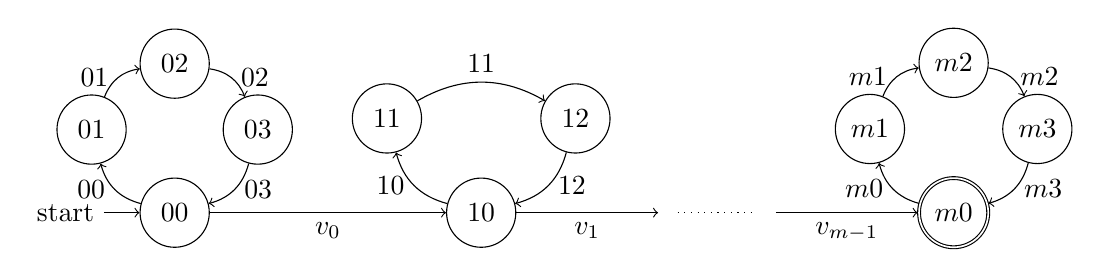
\begin{tikzpicture} 
		\node[state,initial] (q0)  {$\st{0}{0}$};
		\node[state] (q1) [right = 3cm of q0] {$\st{1}{0}$};
		\node (q2) [right = 1.8cm of q1]{};
		\node (q3) [right = 1cm of q2]{};
		\node[state,accepting] (qm) [right = 1.8cm of q3] {$\st{m}{0}$};
		
		\node[state] (q01) [above left = 0.6cm of q0] {$\st{0}{1}$};
		\node[state] (q02) [above = 1cm of q0] {$\st{0}{2}$};
		\node[state] (q03) [above right = 0.6cm of q0] {$\st{0}{3}$};

		\node[state] (q11) [above left = 0.8cm of q1] {$\st{1}{1}$};
		\node[state] (q12) [above right = 0.8cm of q1] {$\st{1}{2}$};

		\node[state] (qm1) [above left = 0.6cm of qm] {$\st{m}{1}$};
		\node[state] (qm2) [above = 1cm of qm] {$\st{m}{2}$};
		\node[state] (qm3) [above right = 0.6cm of qm] {$\st{m}{3}$};

  		\draw[->] (q0) edge [bend left] node [left]{$\sym{0}{0}$} (q01) ;
  		\draw[->] (q01) edge [bend left] node [left]{$\sym{0}{1}$} (q02) ;
  		\draw[->] (q02) edge [bend left] node [right]{$\sym{0}{2}$} (q03) ;
  		\draw[->] (q03) edge [bend left] node [right]{$\sym{0}{3}$} (q0) ;
  		
  		\draw[->] (q0) edge node [below]{$v_0$} (q1) ;
  		\draw[->] (q1) edge node [below]{$v_1$} (q2) ;
  		\draw[dotted] (q2) edge (q3) ;
  		\draw[->] (q3) edge node [below]{$v_{m-1}$} (qm) ;

  		\draw[->] (qm) edge [bend left] node [left]{$\sym{m}{0}$} (qm1) ;
		\draw[->] (qm1) edge [bend left] node [left]{$\sym{m}{1}$} (qm2) ;
		\draw[->] (qm2) edge [bend left] node [right]{$\sym{m}{2}$} (qm3) ;
		\draw[->] (qm3) edge [bend left] node [right]{$\sym{m}{3}$} (qm) ;

  		\draw[->] (q1) edge [bend left] node [left]{$\sym{1}{0}$} (q11) ;
		\draw[->] (q11) edge [bend left] node [above]{$\sym{1}{1}$} (q12) ;
		\draw[->] (q12) edge [bend left] node [right]{$\sym{1}{2}$} (q1) ;
	\end{tikzpicture} 

	\caption{An example of a parametric flat automaton}
	\label{fig:sfa_def}
\end{figure*}

%A finite automaton $D=(Q,T',\Sigma,q_0,q_m)$ is an \emph{instance} of a PFA $S=(Q,T,\cvar,q_0,q_m)$, if there exists an interpretation $I: \cvar \cup \{\epsilon\} \rightarrow \Sigma_\epsilon$ satisfying $I(\epsilon)=\epsilon$ and $T'=\{(q,I(c),q')\mid (q,c,q')\in T\}$. We write $I(S)$ to denote the instance of $S$ wrt. $I$. The language of $S$ is defined as $L(S)= \cup\{L(D) \mid D \mbox{ is an instance of } S\}$. Notice that $L(S)$ is regular because every PFA has only finitely many instance and the finite union of regular languages are also regular.


%Such automata are recognizers of symbolic strings, i.e., strings over $\cvar$.
Parametric automata accept strings over $\cvar$, called \emph{parametric strings}, but we still use them as representations of languages over $\Sigma$. 
%
Namely, string over $\cvar$ are interpreted as strings over $\Sigma$ given an assignment of characters to its character variables.  
%
Formally, an \emph{interpretation $I$ over $\cvar$} is a mapping from $\cvar$ to $\Sigma_\epsilon$ and for a parametric string $x= v_1v_2\cdots v_k$ over $\cvar$, $I(x)$ is defined as $I(v_1)\cdot I(v_2)\cdot \ldots \cdot I(v_k)$.
%
We define the semantics of $x$ as the set $\semof x$ of all possible interpretations of $x$, the semantics of a language $L\subseteq V_\Sigma$ is the union $\semof L = \cup_{x\in L} \semof{x}$ of semantics of its words, and the semantics $\semof A$ of an PFA is the semantics of its language. 

The crucial feature of parametric flat automata is that their semantics can be faithfully represented by a linear integer arithmetic formulae and handled by an SMT solver, allowing to circumvent more costly automata algorithms and decision procedures. \lh{concretize and justify this better?}
%
Achieving this was the purpose of introducing the structural constraints of PFA. 
Their implication central for our method is that every parametric string $x\in L(A)$ is uniquelly determined by its Parikh image $\parikhof{x}$, as formalised by the following lemma.  

\begin{lemma}\label{lemma:parikh}
For an PFA $A$ and $x,y\in L(A)$ if $\parikhof x = \parikhof y$ then $x = y$. 
\end{lemma}
%
Indeed, since every variable appears on at most one transition, then the $\parikhof x$ value of all variables appearing within the same cycle is the same, and it is equal to the number of repetitions of that cycle in the accepting run. 
%
The accepting run on $x$ (and so $x$ itself) can thus be reconstructed from $\parikhof x$. \lh{say precisely how?}
%
For example, in the example of Figure~\ref{fig:sfa_def}, 
from $\parikhwof x {v_0} = \parikhwof x {v_1} = \cdots = \parikhwof x {v_{m-1}}=1$ and $\parikhwof x {v^0_1}=\parikhwof x {v^1_1}=\parikhwof x {v^2_1}=2$ we derive that $x=v_0(v^0_1v^1_1v^2_1)^2v_1\cdots v_{m-1}$. 
We may say that $\parikhof x$ is an encoding of $x$, and define the decoding function $\decode A$ such that $\decode A(\parikhof x) = x$.
It is well known that $\parikhof{A}$ can be computed in the form of a linear arithmetic formula  $\parikhfof{A}$ such that $\modelsof{\parikhfof A} = \parikhof{A}$, in time linear to the size of $A$ \cite{}.
\begin{lemma}\label{lemma:decx}
For a PFA $A$, $L(A) = \{\decode A(\pim) \mid \pim\in\semof{\parikhfof A}\}$.
\end{lemma}


Since every string $w \in \semof{A}$ is obtained from a parametric string $x\in L(A)$ and an interpretation of character varriables $I:\cvar\rightarrow\Sigma_\epsilon$ such that $w = I(x)$, and since $x = \decode A(\parikhof x)$, 
we may say that the assignment $I \cup \parikhof x$ uniting the interpretation $I$ and the Parikh image of the parametric string $x$ encodes $w$. Lemma~\ref{lemma:parikh} also implies that two different strings are encoded by different united assignments (the Parikh image or the interpretation must be different), and hence we may extend the decoding function $\decode A$ to united assignments so that $\decode A(I \cup x) = w$.
Encodings of strings in $\semof{A}$ are encodings of parametric strings of $L(A)$ paired with arbitrary interpretations of character variables $\cvar$, 
hence $\semof A$ is characterised by models of $\parikhof A$ interpreted over variables $\cvar\cup\pvar$ (variables of $\cvar$  may have arbitrary values since $\parikhof A$ does not constraint them), we may say that 
%\begin{lemma}\ref{lemma:decw}
%For a PFA $A$, $\semof{A} = \{\decode(I\cup \pim) \mid \pim\in\semof{\parikhfof A} \land I:\cvar\rightarrow \Sigma_\epsilon\}$.
%\end{lemma}
 $$\semof{A} = \{\decode A(I\cup \pim) \mid I\cup\pim\in\semof{\parikhfof A}_{\cvar\cup\pvar}\}$$
where $\semof{\parikhfof A}_{\cvar\cup\pvar}$ are models of $\parikhfof A$, assignments to $\pvar$, united with arbitrary interpretations of $\cvar$ \lh{this is ugly}.

\paragraph{Synchronisation of PFA}
The following construction of the so called synchronisation formula of two PFA $A$ and $A'$ is a crucial component of building overapproximations of string constraints. 
Synchronisation formula is a formula $\syncfof A {A'}$ over $\pvarone\cup\pvartwo\cup\cvarone\cup \cvartwo$ encoding the semantic intersection $\semof A \cap \semof {A'}$. Besides the intersection, it contains a more precise information about the synchronisation of $A$ and ${A'}$, 
namely, it characterises the set of pairs of encodings $(I\cup \pim)\in \parikhof A$ and $(I'\cup \pim')\in\parikhof {A'}$ such that 
$\decode A(I\cup \pim) = \decode {A'}(I'\cup \pim')$.% which constitute the intersection.

Assume that $A = (Q,T,\cvarone,q_i,q_f)$ and ${A'} = (Q',T',\cvartwo,q_i',q_f')$ are two SFA over disjoint sets of variables, $\cvarone \cap \cvartwo = \emptyset$. 
We build so called asynchronous product automaton $\syncof A {A'}$ of $A$ and ${A'}$ and then extract the formula $\syncfof A {A'}$ from its Parikh image.
%
Such product automaton uses $Q\times Q'$ as the set of states and 
%$(\cvarone \cup \{\epsilon\}) \times (\cvartwo \cup \{\epsilon\} )$ 
$\cvarone_\epsilon\times\cvartwo_\epsilon$
as the alphabet. 
%
Every accepting run of $\syncof A {A'}$ \lh{define run as a sequence of transitions etc} corresponds to an accepting run of $A$ and an accepting run of ${A'}$, and the word accepted by the run of $\syncof A {A'}$ implies a set of constraints on $\pvarone\cup\pvartwo\cup\cvarone\cup\cvartwo$ under which the word accepted by $A$ has the same semantics as the word accepted by ${A'}$.
%
Particularly, if a transition $((q_1,q_1'), (v,v'),(q_2,q_2'))$ is taken, it means the character variable $v$ and $v'$ should be assigned the same value and this value leads $A$ from state $q_1$ to state $q_2$ and ${A'}$ from $q_1'$ to $q_2'$.
%
If a transition $((q_1,q_1'), (v,\epsilon),(q_2,q_1'))$ is taken, then it means that the character variable $v$ should be assigned $\epsilon$, $A$ may transition under $v$ to $q_1$ and ${A'}$ stays in the same state, as a response to $A$s reading epsilon may as well be taking no action. Symmetrically, ${A'}$ might read a variable $v$ assigned $\epsilon$ and $A$ may stay.

Formally, the product automaton is a tuple $\syncof A {A'} = (Q\times Q', \syncT, \cvarone_\epsilon \times \cvartwo_\epsilon, (q_i,q_i'),(q_f,q_f'))$, where the transition relation $\syncT$ is the minimal set satisfying the following:
%
\begin{itemize}
\item If $(q_1,v,q_2) \in T$ and $(q_1',v',q_2') \in T'$, then we have $((q_1,q_1'),(v,v'),(q_2,q_2'))\in \syncT$.
\item If $(q_1,v,q_2) \in T$, then for all states $q'\in Q'$, we have $((q_1,q'),(v,\epsilon),(q_2,q'))\in \syncT$.
\item If $(q_1',v',q_2') \in T'$, then for all states $q\in Q$, we have $((q,q_1'),(\epsilon,v'),(q,q_2'))\in \syncT$.
\end{itemize}	
%
Next, we define the set of constraints that extract from $\syncof A {A'}$ pairs of united assignments (encodings of strings over $\Sigma$) that encode the same string. 
We start with the Parikh formula $\parikhfof {\syncof A {A'}}$ of $\syncof A {A'}$ over the set of variables $\{\#(v,v')\mid (v,v') \in \cvarone_\epsilon \times \cvartwo_\epsilon\}$ of the product automaton and conjoin it with the following restricting constraints. 
%We use $\#v$ and $\#v'$ to denote the number of occurrences of $v_i$ and $v_i^{(j)}$, respectively. 

The first restricting constraint establishes the relation of between the Parikh image of a word accepted by $\syncof A {A'}$ and the Parikh images of the corresponding parametric strings accepted by $A$ and ${A'}$:
$$ \Psi_{\#} = 
\left(\bigwedge_{v\in\cvarone}\#v = \sum_{x' \in \cvartwo_\epsilon} \#{(v,x')}\right)
\land
\left(\bigwedge_{v'\in\cvartwo} \#v' = \sum_{x \in \cvarone_\epsilon} \#{(x,v')}\right)
$$
Notice that $x,x'$ are either variables or $\epsilon$.
%\begin{enumerate}
%	\item for all $v \in \cvarone$, $\#(v) = \sum_{v' \in \cvartwo} \#{(v,v')}$   
%	\item for all $v \in \cvartwo$, $\#(v) = \sum_{v' \in \cvarone} \#{(v',v)}$ 
%\end{enumerate}

Then we add the following linear constraints to enforce that the decodings of the models are indeed the same, 
% condition 1. and 2. required for the pair of symbolic string $(w_n, w_m)$ and $I$, i.e., $I(w_n) = I(w_m)$ and $I$ assign the same value to all versions of the same variable (we use $-1$ as the value of $\epsilon$). 
$$ \Psi_= =
\bigwedge_{x\in\cvarone_\epsilon,x'\in\cvartwo_\epsilon} \#(x,x')>0 \rightarrow (x=x')
$$
%\begin{enumerate}
%	\item for all $v\in \cvarone$ and $v'\in \cvartwo$, $\#{(v,v')}>0 \rightarrow (v=v')$, 
%	\item for all $v\in \cvarone$, $\#{(v,\epsilon)}>0 \rightarrow (v=\epsilon)$, and
%	\item for all $v\in \cvartwo$,$\#{(\epsilon,v')}>0 \rightarrow (v'=\epsilon)$.
%\end{enumerate}

The synchronisation formula is the conjunction 
$$
\syncfof A {A'} = \parikhfof{\syncof A {A'}} \land \Psi_{\#} \land \Psi_=
$$
The correctness of this construction is expressed by the following lemma
%\begin{lemma}
%For $\pim:\pvarone\rightarrow \nat$, $\pim':\pvartwo \rightarrow\nat$, $I:\cvarone\rightarrow\Sigma$, $I':\cvartwo\rightarrow\Sigma$, 
%we have $(I\cup\pim)\cup(I'\cup\pim')\in\semof {\syncfof A {A'}}$ if and only if $\decode A(I\cup\pim) = \decode {A'}(I'\cup\pim')$.
%\end{lemma}

\begin{lemma}
 $\semof {\syncfof A {A'}} = \{(I\cup\pim)\cup(I'\cup\pim') \mid \decode A(I\cup\pim) = \decode {A'}(I'\cup\pim')\}$. 
\end{lemma}

We actually have even something stronger, namely, that, $\syncfof A {A'}$ has all possible allignments. How do I say this ... or do I have to say this?


\begin{lemma}
	Symbolic flat automata are closed under concatenation.
\end{lemma}






\subsection{Flat Under-approximation for Equalities and Regular Constraints} \label{section:eq}

Given an equality constraint $x_1\cdot x_2 \cdots x_n = x_{n+1}\cdot x_{n+2} \cdots x_m$, we restrict the domain of all variables to some PFA with disjoint alphabet and then connect the final state and initial state of two consecutive variables with an epsilon transition. We rename the variables on the transitions of PFA's for different occurrences of the same variable in one equality constraint. Later we will use some arithmetic constraints to enforce that all occurrences of the variants of the same variable will be assigned the same value. For notational convenience, the renaming is done by adding a version number to the variable. For example, we can rename $v_1$ to $v_1^{(0)}$, $v_1^{(1)}$, $\ldots$.

For the constraint $xy = yx$, we first restrict the domains of $x$ and $y$ to the PFA in Figure~\ref{fig:sfa} (a) and (b), respectively. In the construction of the PFA for $xy$ and $yx$ (Figure~\ref{fig:sfa} (c) and (d)), we rename the variables on the PFA of $X$ and $Y$ to some fresh variable for each different occurrence of $x$ and $y$ in $xy = yx$.

\begin{figure*}
	\tikzset{state/.style={circle,draw=blue!50,fill=blue!20,
			thick,inner sep=0pt,minimum size=6mm}, initial text=$ $}
		
 	\begin{minipage}[t]{0.15\textwidth} 
	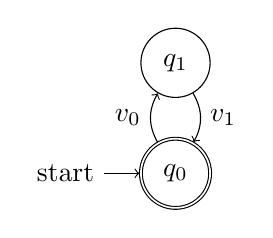
\begin{tikzpicture}
	\node[state,initial,accepting] (q0)  {$q_0$};
	
	\node[state] (q01) [above = 0.5cm of q0] {$q_1$};

	\draw[->] (q0) edge [bend left] node [left]{$v_0$} (q01) ;
	\draw[->] (q01) edge [bend left] node [right]{$v_1$} (q0) ;
	\end{tikzpicture} 
	
	\centering
	(a) $A_x$
	\end{minipage}
 	\begin{minipage}[t]{0.15\textwidth} 
	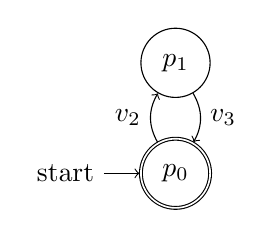
\begin{tikzpicture} 
	\node[state,initial,accepting] (q0)  {$p_0$};
	
	\node[state] (q01) [above = 0.5cm of q0] {$p_1$};
	
	\draw[->] (q0) edge [bend left] node [left]{$v_2$} (q01) ;
	\draw[->] (q01) edge [bend left] node [right]{$v_3$} (q0) ;
	\end{tikzpicture} 
	
	\centering
	(b) $A_y$
	\end{minipage}
	\begin{minipage}[t]{0.28\textwidth}
	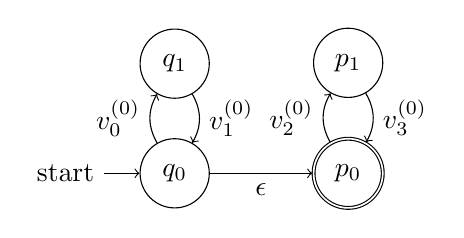
\begin{tikzpicture} 
	\node[state,initial] (q0)  {$q_0$};
	\node[state,accepting] (q1) [right = 1.3cm of q0] {$p_0$};
	
	\node[state] (q01) [above = 0.5cm of q0] {$q_1$};

	\draw[->] (q0) edge [bend left] node [left]{$v_0^{(0)}$} (q01) ;
	\draw[->] (q01) edge [bend left] node [right]{$v_1^{(0)}$} (q0) ;
	
	\node[state] (q11) [above = 0.5cm of q1] {$p_1$};
	
	\draw[->] (q1) edge [bend left] node [left]{$v_2^{(0)}$} (q11) ;
	\draw[->] (q11) edge [bend left] node [right]{$v_3^{(0)}$} (q1) ;
	\draw[->] (q0) edge  node [below]{$\epsilon$} (q1) ;
	\end{tikzpicture}
	
	\centering
	(c) $A_{xy}$
	\end{minipage}
	\ \ \ 
	\begin{minipage}[t]{0.28\textwidth}
	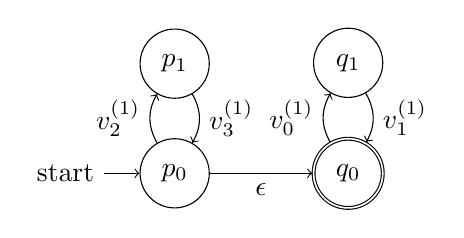
\begin{tikzpicture} 
	\node[state,accepting] (q0)  {$q_0$};
	\node[state,initial] (q1) [left = 1.3cm of q0] {$p_0$};
	
	\node[state] (q01) [above = 0.5cm of q0] {$q_1$};
	
	\draw[->] (q0) edge [bend left] node [left]{$v_0^{(1)}$} (q01) ;
	\draw[->] (q01) edge [bend left] node [right]{$v_1^{(1)}$} (q0) ;
	
	\node[state] (q11) [above = 0.5cm of q1] {$p_1$};
	
	\draw[->] (q1) edge [bend left] node [left]{$v_2^{(1)}$} (q11) ;
	\draw[->] (q11) edge [bend left] node [right]{$v_3^{(1)}$} (q1) ;
	\draw[->] (q1) edge  node [below]{$\epsilon$} (q0) ;
	\end{tikzpicture}
	
	\centering
	(d) $A_{yx}$
	\end{minipage}

	\caption{Symbolic flat automata of $x$, $y$, $xy$ and $yx$}
	\label{fig:sfa}
\end{figure*}

Assume that $S_n=(Q,T,\cvarone,q_i,q_f)$ is the SFA of $x_1\cdot x_2 \cdots x_n$ and $S_m=(P,T',\cvartwo,p_i,p_f)$ is the SFA of $x_{n+1}\cdot x_{n+2} \cdots x_m$. Our next task is to find a model for $x_1\cdot x_2 \cdots x_n = x_{n+1}\cdot x_{n+2} \cdots x_m$ under the domain restriction specified by $S_n$ and $S_m$. 
Note that $\cvarone \cap \cvartwo =\emptyset$, because all variables will be renamed to some fresh variable. 


This is equivalent to finding a pair of symbolic strings $(w_n,w_m) \in L(S_n)\times L(S_m)$ and a common interpretation $I$ such that 
\begin{enumerate}
	\item $I(w_n)=I(w_m)$
	\item $I$ assign to variants of the same variable the same value. For example, in Figure~\ref{fig:sfa} (c) and (d), $v_0^{(0)}$ and $v_0^{(1)}$ should be assigned the same value.
	\item different versions of the same variable should occurs equally often in $w_n\cdot w_m$. For example, in Figure~\ref{fig:sfa} (c) and (d), $w_{xy}=v_0^{(0)}v_1^{(0)}v_0^{(0)}v_1^{(0)}$ and $w_{yx}=v_0^{(1)}v_1^{(1)}v_0^{(1)}v_1^{(1)}$ is a pair of symbolic strings satisfying this condition. The number of occurrences of $v_i^{(0)}$ is the same to $v_i^{(1)}$ for $i\in[0,1]$ in the concatenation $w_{xy}\cdot w_{yx}$.
	But the pair $v_0^{(0)}v_1^{(0)}v_0^{(0)}v_1^{(0)}$ and $v_2^{(0)}v_3^{(0)}v_2^{(0)}v_3^{(0)}$ does not satisfy the condition. Observe that $v_0^{(0)}$ occurs twice, but $v_0^{(1)}$ is not there.
\end{enumerate}

In order to find such a pair of symbolic strings $(w_n,w_m) \in L(S_n)\times L(S_m)$ and an interpretation $I$, we first build a ``product'' automaton of $S_n$ and $S_m$ and then add some additional linear arithmetic constraints to enforce the above conditions.

Such product automaton uses $Q\times P$ as the set of states and 
%$(\cvarone \cup \{\epsilon\}) \times (\cvartwo \cup \{\epsilon\} )$ 
$\cvarone\times\cvartwo$
as the alphabet. If a transition $((q_1,p_1), (v,v'),(q_2,p_2))$ is taken, it means the character variable $v$ and $v'$ should be assigned the same value and this value leads $A$ from state $q_1$ to state $q_2$ and $B$ from $p_1$ to $p_2$.

More precisely, the product automaton is a tuple $\syncof A B = (Q\times P, \syncT, (\cvarone \cup \{\epsilon\}) \times (\cvartwo \cup \{\epsilon\} ), (q_i,p_i),(q_f,p_f))$, where the transition relation $\syncT$ is the minimal set satisfying the following.

\begin{itemize}
\item If $(q_1,v_i^{(j)},q_2) \in T$, then for all states $p\in P$, we have $((q_1,p),(v_i^{(j)},\epsilon),(q_2,p))\in \syncT$.
\item If $(p_1,v_i^{(j)},p_2) \in T'$, then for all states $q\in Q,((q,p_1)$, we have $(\epsilon,v_i^{(j)}),(q,p_2))\in \syncT$.
\item If $(q_1,v_i^{(j)},q_2) \in T$ and $(p_1,v_{i'}^{(j')},p_2) \in T'$, then we have $((q_1,p_1),(v_i^{(j)},v_{i'}^{(j')}),(q_2,p_2))\in \syncT$.
\end{itemize}	
The first two cases correspond to the situation when the character variable $v_i^{(j)}$ is assigned $\epsilon$. In such cases, only one automaton changes its state.

For example, in the product automaton $A_{xy=yx}$ corresponds to $xy=yx$, we have the following transitions
\begin{itemize}
	\item $((q_0,p_0), (v_0^{(0)},\epsilon),(q_1,p_0))$, because $(q_0,v_0^{(0)},q_1)$ is a transition of $A_{xy}$.
	\item $((q_0,p_0), (\epsilon,\epsilon),(q_0,q_0))$, because $(p_0,\epsilon,q_0)$ is a transition of $A_{yx}$.
	\item $((q_0,p_0), (v_0^{(0)},v_2^{(1)}),(q_1,q_1))$, because $(q_0,v_0^{(0)},q_1)$ is a transition of $A_{xy}$ and $(p_0,v_2^{(1)},p_1)$ is a transition of $A_{yx}$.
\end{itemize}

Recall that for flat automata, the number of occurrences of each symbol uniquely characterizes an accepting string (Section~\ref{section:sfa}) and for any finite automaton we can construct a Presburger formula characterizing its Parikh image (Section~\ref{section:preliminary}). For a product automaton $A$ computed from the previous step, we compute a Presburger formula $\phi(A)$ over the set of variables $\{\#{(v_i^{(j)},v_{i'}^{(j')})}\mid (v_i^{(j)},v_{i'}^{(j')}) \in \cvarone \times \cvartwo\}$ characterizing the Parikh image of $A$. We use $\#(v_i)$ and $\#(v_i^{(j)})$ to denote the number of occurrences of $v_i$ and $v_i^{(j)}$, respectively. The following formulae establish the relation of the number of occurrences of symbols between the SFAs and the product automaton.
\begin{enumerate}
	\item for all $v_i^{(j)} \in \cvarone$, $\#(v_i^{(j)}) = \sum_{v \in {\cvartwo \cup \{\epsilon\}}} \#{(v_i^{j},v)}$   
	\item for all $v_i^{(j)} \in \cvartwo$, $\#(v_i^{(j)}) = \sum_{v \in {\cvarone \cup \{\epsilon\}}} \#{(v,v_i^{j})}$ 
\end{enumerate}

Then we add the following linear constraints to enforce  condition 1. and 2. required for the pair of symbolic string $(w_n, w_m)$ and $I$, i.e., $I(w_n) = I(w_m)$ and $I$ assign the same value to all versions of the same variable (we use $-1$ as the value of $\epsilon$). 
\begin{enumerate}
	\item for all $v_i^{(j)}\in \cvarone$ and $v_{i'}^{(j')}\in \cvartwo$, $\#{(v_i^{(j)},v_{i'}^{(j')})}>0 \rightarrow (v_i=v_{i'})$,\lh{typo?} 
	\item for all $v_i^{(j)}\in \cvarone$, $\#{(v_i^{(j)},\epsilon)}>0 \rightarrow (v_i=\epsilon)$, and
	\item for all $v_{i'}^{(j')}\in \cvartwo$,$\#{(\epsilon,v_{i'}^{(j')})}>0 \rightarrow (v_{i'}=\epsilon)$.
\end{enumerate}
We then add the linear constraints $\#(v_i) = \#(v_i^{(j)})$, for all $v_i\in \cvar$ and all different version numbers $j$ for $v_i$, to enforce condition 3, which says different versions of the same variable should occurs equally often in $w_n\cdot w_m$. 

From the model $M$ of the linear constraints, we can obtain $w_n$, $w_m$, and $I$. The interpretation $I$ is defined as $I(v)=M(v)$ for all $v\in (\cvarone \cup \cvartwo)$. The symbolic words $w_n$ and $w_m$ can be obtained by traverse the SFAs following the number of occurrences of each character variables.
More specifically, assume that the SFA $S_n$ is the one in Figure~\ref{fig:sfa_def}, then $$w_n = (v_0^0v_0^1v_0^2v_0^3)^{\#(v_0^0)}v_0(v_1^0v_1^1v_1^2)^{\#(v_1^0)}v_1\ldots(v_m^0v_m^1v_m^2v_m^3)^{\#(v_m^0)}$$
Note that $\#(v_0^0)=\#(v_0^1)=\#(v_0^2)=\#(v_0^3)$, so we just use $\#(v_0^0)$ to denote the number of times of first loop traversal. One can construct $w_m$ in a similar way. Using the same approach, one can derive the assignment to variables in $\vars$ using the corresponding count and values of variables in $\cvar$.

Disequality constraint $x_1\cdot x_2 \cdots x_n \neq x_{n+1}\cdot x_{n+2} \cdots x_m$ can be converted to equal-satisfiable equality constraints in the standard way~\cite{abdulla2015norn}. We replace it with the following constraints.

$$
\begin{array}{c}
(|x_1|+ |x_2|+ \cdots +|x_n| \neq |x_{n+1}| + |x_{n+2}|+ \cdots +|x_m|)\vee \\
\left(
	\begin{array}{cccc}
	
	 y_1\cdot y_2\cdot y_3 &=& x_1\cdot x_2 \cdots x_n &\wedge\\
	 y_1 \cdot y'_2 \cdot y'_3 &=& x_{n+1}\cdot x_{n+2} \cdots x_m &\wedge\\
	|y_2|&=&|y'_2|=1
	\end{array}

\right)
\end{array}
$$

The second disjunct says that the constraints $x_1\cdot x_2 \cdots x_n$ and $x_{n+1}\cdot x_{n+2} \cdots x_m$ have a common prefix $y_1$, but the next character $y_2$ and $y'_2$ is different. In an more efficient implementation, one just project $y_2$ and $y'_2$ to a SFA that accept only symbolic words $v_1$ and $v'_1$, respectively (the SFA has no loop and only one transition). 



\todo{Maybe talk about the heuristic that we merge the list elements into one}





%%%%%%%%%%%%%%%%%%%%%%%%%%%%%%%%%%%%%%%%%%%%%%%%%%%%%%%%%%%%%%%%%%%%%%%%%%%%%%
\subsection{Handling String-Integer Conversion} \label{section:s2i}
%%%%%%%%%%%%%%%%%%%%%%%%%%%%%%%%%%%%%%%%%%%%%%%%%%%%%%%%%%%%%%%%%%%%%%%%%%%%%%

In this section, we discuss how to handle the constraint $n=\sti{x}$ by restricting the domain of $x$ to some SFA. Let us begin with a simple example, assume that we use the SFA in Figure~\ref{fig:sfa} (a) to restrict the domain of $x$. Then we know that when $0\leq v_0,v_1 \leq 9$, then $n$ is a positive integer value, and otherwise $n =-1$. So we should first add the constraint $ ((0\leq v_0\leq 9) \wedge (0\leq v_1\leq 9)) \vee n=-1 $.

For the case that $n$ is a positive integer, the value of $n$ can be characterized by a constraint $n= (v_0\times 10+ v_1) \times (1+100 +100^2 + \ldots 100 ^{\#(v_0)-1})=  (v_0\times 10+ v_1) \times \frac{100^{\#(v_0)}-1}{100-1}$. 
The constraint uses $\#(v_0)$ to capture the total number of loop traversal.
Notice that the constraint above contains an exponential component $\frac{100^{\#(v_0)}}{100-1}$. To solve the satisfiability of this formula, one need to solve an exponential constraint. 

Let us have a look at another example. If we restrict the domain of $x$ to the SFA in Figure~\ref{fig:sfa} (c), for the case when $n$ is positive, we have the relation $n= (v_0^{(0)}\times 10+ v_1^{(0)}) \times (1+100 +100^2 + \ldots 100 ^{\#(v_0^{(0)})-1})\times 100^{\#(v_2^{(0)})}+(v_2^{(0)}\times 10+ v_3^{(0)}) \times (1+100 +100^2 + \ldots 100 ^{\#(v_2^{(0)})-1}) =  (v_0^{(0)}\times 10+ v_1^{(0)}) \times \frac{100^{\#(v_0^{(0)})}-1}{100-1}\times 100^{\#(v_2^{(0)})} + (v_2^{(0)}\times 10+ v_3^{(0)}) \times \frac{100^{\#(v_2^{(0)})}-1}{100-1}$. Observe that the formula has two exponential components $\frac{100^{\#(v_0^{(0)})}\times 100^{\#(v_2^{(0)})} }{100-1}$ and $\frac{100^{\#(v_2^{(0)})} }{100-1}$.

It is not difficult to observe that, for the case of an arbitrary SFA of $m$ loops, the formula to define $n$ contains $m$ exponential components, one for each loop.
To the best of our knowledge, the satisfiability problem of integer constraints with a mix of polynomials and exponentials is still open. As said in the introduction, the problem is difficult even for the case that variables are real numbers. For example, the algorithm in~\cite{kincaid2019closed} involves a quantifier elimination procedure, which is double-exponential to the length of the input formula and hence cannot handle large instances. So we do not expect that this constraint can be solved efficiently.

\paragraph{SFA that allows efficient string-integer conversion: } In the previous discussion, we know that it is unlikely to use arbitrary SFA and gain efficient solving procedure, due to the requirement to solve exponential integer constraints. The problem is that each loop in the SFA creates an exponential component. An immediate idea would be that maybe we can restrict the variable to some specific SFA that allow more efficient constraint solving. At the same time, we want to keep some good property, i.e., the search space covers all integers with at most $m$-digits.

Our first attempt is a SFA with no loop, i.e., a straight line structure (e.g., the SFA in Fig~\ref{fig:sfa_its} without the self-loop at $q_0$). The corresponding integer constraint does not have exponential components. However, it does not ensure the property that all numbers with at most $m$-digits are covered. Consider the example $\sti{x}=10 \wedge |x|=5$. The number $10$ has only $2$-digits, at the first glance, a straight-line SFA with two transitions, i.e., the SFA \scalebox{0.5}{\tikzset{state/.style={circle,draw=blue!50,fill=blue!20,
			thick,inner sep=0pt,minimum size=6mm}, initial text=$ $}
	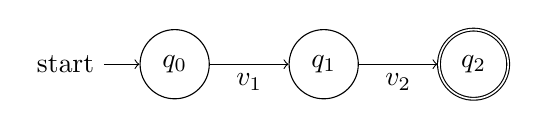
\begin{tikzpicture} 
	\node[state,initial] (q0)  {$q_0$};
	\node[state] (q1) [right = 1cm of q0] {$q_1$};
	\node[state,accepting] (q2) [right = 1cm of q1] {$q_2$};
	
	\draw[->] (q0) edge node [below]{$v_1$} (q1) ;
	\draw[->] (q1) edge node [below]{$v_2$} (q2) ;
	\end{tikzpicture}}, should be sufficient for the domain restriction of $x$. If we do so, we will conclude that the formula is unsatisfiable, because the length of $x$ cannot be $5$  under this domain restriction.

However, the formula is satisfiable when $x=``00010"$. Observe that $\sti{``00010"}=10$. The key is that even for a bounded integer, the corresponding string can be of unbounded length with arbitrarily many `$0$' characters at the front. In order to handle all number with at most $m$ digits, we propose to restrict the domain of $x$ to a SFA in Figure~\ref{fig:sfa_its}.  The SFA has a self-loop transition labeled $v_0$ at $q_0$ and we always add a constraint $v_0=0$ for such SFA. With this transition, we can ensure that the under-approximation handles all numbers with at most $m$ digits. Although this SFA still has a loop, but it will not create any exponential component because the loop only represents a sequence of `0' that occurs in the prefix of $x$. It will not affect the integer value of $n=\sti{x}$.

\begin{figure}
	\tikzset{state/.style={circle,draw=blue!50,fill=blue!20,
			thick,inner sep=0pt,minimum size=6mm}, initial text=$ $}
	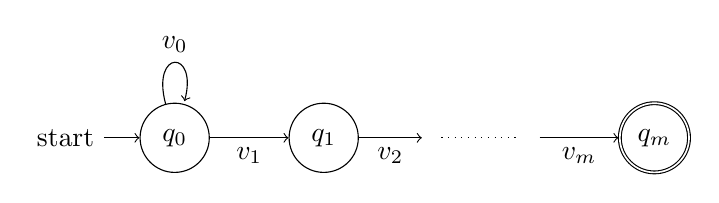
\begin{tikzpicture} 
	\node[state,initial] (q0)  {$q_0$};
	\node[state] (q1) [right = 1cm of q0] {$q_1$};
	\node (q2) [right = 0.8cm of q1]{};
	\node (q3) [right = 1cm of q2]{};
	\node[state,accepting] (qm) [right = 1cm of q3] {$q_m$};
	
	\draw[->] (q0) edge node [below]{$v_1$} (q1) ;
	\draw[->] (q1) edge node [below]{$v_2$} (q2) ;
	\draw[dotted] (q2) edge (q3) ;
	\draw[->] (q3) edge node [below]{$v_m$} (qm) ;
	\path (q0) edge [loop above] node {$v_0$} (q0);
	\end{tikzpicture} 
	
	\caption{An example of a symbolic flat automaton}
	\label{fig:sfa_its}
\end{figure}

Such SFA handles bounded integers (e.g., 10-digits or 64-bits) precisely and under-approximate the possible values of unbounded integers. It works very efficiently because we just need to use linear constraints to characterize the relation between $x$ and $n$. 
Remember that the character variables can be assigned $\epsilon$. In order to handle such cases efficiently, we use an encoding that if $v_j = \epsilon = -1$ then $v_k = -1$ for all $k\in [j,m]$, i.e., we shift all the $\epsilon$-transitions to the least significant digits. In order to explain this encoding, we first define two macro function:

$$\begin{array}{rl}
\mathsf{epsilonAfter(k)}::=& (0\leq v_0,\ldots, v_k\leq 9) \wedge\\
&v_{k+1}=\ldots =v_m = -1\\
\mathsf{toNumber(k)}::=& (n = v_0\times 10^{k} + v_1\times 10^{k-1} + \ldots + v_{k})
\end{array}
$$

The function $\mathsf{epsilonAfter(k)}$ forces the first $k$ variables to be assigned some number and those after $k$ be assigned $\epsilon$. Recall that we use $-1$ to represent $\epsilon$. The function $\mathsf{toNumber(k)}$ converts the first $k$ variables to the corresponding number in $n$.
Then we can specify the relation between $n$ and the character variables as follows:
$$(n=-1 \vee \bigvee_{k\in [0,m]} (\mathsf{epsAfter(k)} \wedge \mathsf{toNumber(k)} ) )$$
It says either $x$ is not a number and so $n=-1$ or the first $k$ variables represent the value of $n$, for some $k\in [0,m]$ .


\hide{The length of $x$ can be specified by the following formula.

$\begin{array}{ccc}
	(|x|&=& \#(v_0)+1 \wedge 0\leq v_1 \leq 9 \wedge v_2 = -1)\vee \\
	(|x|&=& \#(v_0)+2 \wedge 0\leq v_2 \leq 9 \wedge v_3 = -1)\vee \\
	& &\ldots\\
	(|x|&=& \#(v_0)+(m-1) \wedge 0\leq v_{m-1} \leq 9 \wedge v_m = -1)\vee\\
	(|x|&=& \#(v_0)+m \wedge 0\leq v_m \leq 9 )
\end{array}$}

\todo{Add an example: $\sti{x}=\sti{y} \wedge x= y\cdot y$. Do product construction informally here.}

% \section{Evaluation}
%  \label{section:evaluation}
% \todo{copy a few tables from our test site to here}

\section{Implementation}
\section{Implementation and Evaluation}
\label{section:evaluation}

We have implemented our string constraint solving procedure in a tool called {\tool}. {\tool} is implemented as a theory solver of the SMT solver Z3~\cite{z3}. In this way, we can concentrate on solving conjunctive constraints and let Z3 handle the other boolean connectives. Secondly, it makes it possible to solve not only formulae over string constraints but also combinations of string constraints with other theories that Z3 supports. Furthermore, this approach allows us to more effectively handle the arithmetic constraints that are generated by the under-approximation module and, lastly, it eliminates the need to have our own parser. 

In {\tool}, we use the following PFA selection strategy. We use \emph{numeric PFAs} for string variables appearing in string-number conversion and \emph{standard PFAs} for others. We select a size $m$ for numeric PFAs, a number $p$ of their loops, and the length $q$ of the loops. Initially, we set $(m,p,q)=(5,2,q)$ where $q$ is dynamic and obtained from our internal static analysis. We double $m$ and increase $p$ and $q$ by one if refinement is required. We set an upper bound for each parameter and report UNKNOWN if a solution cannot be found within the bound.

Our over-approximation module also uses heuristics to derive the constant value of any side of the constraint $n=\sti{x}$ to refine the over-approximation. For instance, assume we can derive that $n=12$ from some integer constraints. Then we can derive the value of $x$ belongs to the regular language $(0^*12)$. 
%HERE

%more or less standard
The way our theory solver and Z3 interact is almost standard. When Z3 asks our theory solver a string constraint satisfiability problem, our solver tries to prove it is SAT or UNSAT using the procedure discussed in this paper. For under-approximation, whenever a corresponding linear formula is created, we attach the current value of $m$, $p$, $q$ to the formula, and then push it to Z3 core. If our theory solver reports UNKNOWN, Z3 remembers it in a global flag \textsf{incomplete} and either tries another solution branch, or the same solution branch with different value of $m$, $p$, $q$. If Z3 completes the search of all solution branches, it reports UNSAT if the flag \textsf{incomplete} is down, and UNKNOWN otherwise.


We compare {\tool} \changed{(\texttt{1e715b7dab})} with other state-of-the-art string solvers, namely, CVC4~(45bcf28ab)~\cite{cvc4Tool}, and Z3~(\texttt{d95b549ff})~\cite{z3}, \textsf{Z3Str3}~(\texttt{d95b549ff})~\cite{zheng2013z3}. For these tools, we use the GitHub version stated in the parenthesis because their performance are in general better than the corresponding release version. \changed{Observe that CVC4 and Z3 are  DPLL(T)-based string solvers.}
We do not compare with Sloth \cite{sloth} since it does not support length constraints, which occur in most of our benchmarks. We also do not compare with ABC~\cite{aydin2018parameterized} (a model counter for string constraints), Ostrich~\cite{chen2019decision} and \textsf{Trau+}~\cite{abdulla2019chain}, because they do not support many of the string functions in our benchmarks, especially string-number conversion.

We perform two sets of experiments. In the first set of experiments, we compare {\tool} with other tools on existing benchmarks over basic string constraints. Those benchmarks do not involve string-number conversion functions. In the second set of experiments, we compare {\tool} with the other tools on new suites focusing on string-number conversion. Our goals of experiments are the following:
\smallskip


\begin{itemize}
	\item {\tool} performs as good as or better than the other tools in solving the  satisfiability problems of basic string constraints.
	
		\smallskip

	\item {\tool} performs significantly better than the other tools in solving the satisfiability problems on string-number conversion benchmark, and this shows  the efficiency of PFA in general and \emph{numeric} PFA in particular.
\end{itemize}
		\smallskip

In the first set of experiments, we use the following benchmark examples:

		\smallskip


\begin{itemize}
	\item PyEx~\cite{pyex} comes from running the symbolic executor PyEx over some Python packages.
	
	\smallskip
	
	
%	\item APLAS~\cite{aplas} includes 600 hand-drafted tests consisting of only equality and integer length constraints.
	
	
	%	\smallskip


	\item \changed{ LeetCode comes from running PyEx over a sample code collected from the LeetCode~\cite{LeetCode} website, including functions that check whether a string is a valid IPv4 or IPv6 address, sum up two binary numbers, check whether an input string is an abbreviation of another input string, and convert a sequence of digits to a string according to a given mapping.}
	
		\smallskip

	\item StringFuzz~\cite{blotsky2018stringfuzz}  is generated by the fuzz testing tool of the same name.
	
		\smallskip

	\item $\text{cvc4}_{\text{pred}}$ and $\text{cvc4}_{\text{term}}$ are obtained from the CVC4 group~\cite{termEQ}. These benchmarks contain a small amount of string-number conversion constraints (< $5\%$).
\end{itemize}

In the second experiment, we compare with tools supporting string-number conversion on the benchmarks collected from the symbolic executor \texttt{Py-Conbyte}\footnote{\url{https://github.com/spencerwuwu/py-conbyte}}, which has the supports of string-number conversion. We ran it on several examples collected from the LeetCode platform and from Python core libraries, which involve diverse usages of string-number conversion in Python such as parsing date-time, verifying and restoring IP addresses from strings, etc. We also have examples that encode execution paths of some JavaScript programs (the Luhn algorithm and some array manipulations).

	\changed{All experiments were executed on a machine with 4-core CPU, 16 GiB RAM, and MacOS 10.15.4.} The timeout was set to 10s for each test.
We use the results from {\tool}, CVC4, and Z3 as the reference answer for the validation of the correctness of the results. Occasionally, two of them report inconsistent  answers (one SAT and one UNSAT). To decide which solver is right, we developed a validator. It takes the model $I$ returned from the solver who reported SAT, assigns $I(x)$ to all variables $x$ in the test to obtain a modified test, and re-evaluates the modified test by multiple solvers. If the results from all solvers are consistent, we mark the test SAT or UNSAT according to the results. Otherwise, we manually simplify and inspect the test until we get a conclusive result. 

\changed{The results of the experiments are summarized in Table~\ref{table:base_benchmark}, Table~\ref{table:str_int_benchmark}, and Table~\ref{table:checkLuhn}. Rows with heading \texttt{SAT}/\texttt{UNSAT} show numbers of solved formulae. Rows with heading \texttt{UNKNOWN} or \texttt{TIMEOUT} indicate the number of instances for which the solver fails to return an answer. \texttt{ERROR} means system crashes due to various reasons (usually out of memory). \texttt{INCORRECT} shows the number of cases where the tool gives a wrong answer.}


\begin{table}[h]
\changed{
\centering
\caption{Results of {\tool}, CVC4, Z3, and Z3Str3 on Basic String Constraint benchmarks.}
\scalebox{0.85}{
\begin{tabular}{|l r | r r r r |}
\hline
\multicolumn{2}{|c}{}                  & {\tool} & CVC4  &Z3 & Z3Str3 \\ \hline
\multirow{6}{*}{PyEx}		& SAT      & 21377& 19899& 16331&  3037 \\
							& UNSAT    &  3860&  3848&  3831&  3816 \\
							& UNKNOWN  &     0&     0&     0&     7 \\
							& TIMEOUT  &   184&  1674&  5259& 16872 \\
							& ERROR    &     0&     0&     0&  1675 \\
							& INCORRECT&     0&     0&     0&    14 \\ \hline
%\multirow{6}{*}{APLAS}		& SAT      &   126&    51&    13&    35 \\
%							& UNSAT    &   286&   214&   100&   111 \\
%							& UNKNOWN  &     0&     0&     0&   345 \\
%							& TIMEOUT  &   188&   335&   487&    89 \\
%							& ERROR    &     0&     0&     0&    20 \\
%							& INCORRECT&     0&     0&     0&     0 \\ \hline
\multirow{6}{*}{LeetCode}	& SAT      &   877&   865&   881&   661 \\
							& UNSAT    &  1785&  1785&  1785&  1780 \\
							& UNKNOWN  &     0&     0&     0&   122 \\
							& TIMEOUT  &    0&    16&     0&    90 \\
							& ERROR    &     4&     0&     0&    13 \\
							& INCORRECT&     0&     0&     0&     0 \\ \hline
\multirow{6}{*}{StringFuzz}	& SAT      &   515&   704&   267&   505 \\
							& UNSAT    &   301&   245&   188&   192 \\
							& UNKNOWN  &     0&     0&     0&     4 \\
							& TIMEOUT  &   249&   116&   610&   364 \\
							& ERROR    &     0&     0&     0&     0 \\
							& INCORRECT&     0&     0&     0&     0 \\\hline
\multirow{6}{*}{cvc4\textsubscript{pred}} & SAT &    13&    11&    12&     8 \\
							& UNSAT    &   822&   818&   808&   774 \\
							& UNKNOWN  &     0&     0&     0&     4 \\
							& TIMEOUT  &     0&     6&    15&    38 \\
							& ERROR    &     0&     0&     0&     11 \\
							& INCORRECT&     0&     0&     0&     0 \\ \hline
\multirow{6}{*}{cvc4\textsubscript{term}} & SAT &    10&     8&     5&    2 \\
							& UNSAT    &  1032&  1025&  1022&   957 \\
							& UNKNOWN  &     0&     0&     0&     3 \\
							& TIMEOUT  &     3&    12&    18&    58 \\
							& ERROR    &     0&     0&     0&     11 \\
							& INCORRECT&     0&     0&     0&    14 \\ \hline \hline
\multirow{6}{*}{Total} 		& SAT      & 22792& 21487& 17496&  4213\\
							& UNSAT    &  7800&  7721&  7634&  7519\\
							& UNKNOWN  &     0&     0&     0&   140\\
							& TIMEOUT  &  436&  1824&  5902& 17422 \\
							& ERROR    &     4&     0&     0&  1710\\
							& INCORRECT&     0&     0&     0&    28 \\\hline
\end{tabular}}
\label{table:base_benchmark}}
\end{table}

\begin{table}[h]
\changed{
\centering
\caption{Results of {\tool}, CVC4, Z3, and Z3Str3 on String-Number Conversion benchmark.}
\scalebox{0.8}{
\begin{tabular}{|l r | r r r r|}
\hline
\multicolumn{2}{|c}{}          			   & {\tool} &  CVC4 &    Z3 & Z3Str3 \\ \hline
\multirow{6}{*}{Leetcode}		& SAT      &  2501&  1721&  1898&   239 \\ 
								& UNSAT    & 16394& 15726& 16115& 15288 \\
								& UNKNOWN  &     0&     0&     0&   623 \\
								& TIMEOUT  &    32&  1480&   914&  2337 \\
								& ERROR    &     0&     0&     0&   332 \\
								& INCORRECT&     0&     0&     0&   108 \\ \hline 
\multirow{6}{*}{PythonLib}		& SAT      &  1922&   579&   914&   206 \\ 
								& UNSAT    &   724&   667&   724&   642 \\
								& UNKNOWN  &     0&     0&     0&    45 \\
								& TIMEOUT  &     0&  1400&  1008&  1710 \\
								& ERROR    &     0&     0&     0&    41 \\
								& INCORRECT&     0&     0&     0&     2 \\ \hline
\multirow{6}{*}{JavaScript}		& SAT      &    20&     3&    16&     4 \\ 
								& UNSAT    &     0&     0&     0&     0 \\
								& UNKNOWN  &     0&     9&     0&     0 \\
								& TIMEOUT  &     0&     8&     4&    10 \\
								& ERROR    &     0&     0&     0&     6 \\
								& INCORRECT&     0&     0&     0&     0 \\ \hline \hline
\multirow{6}{*}{Total}			& SAT      &  4443&  2303&  2828&   449 \\ 
								& UNSAT    & 17118& 16393& 16839& 15930 \\
								& UNKNOWN  &     0&     9&     0&   668 \\
								& TIMEOUT  &    32&  2888&  1926&  4057 \\
								& ERROR    &     0&     0&     0&   379 \\
								& INCORRECT&     0&     0&     0&   110 \\ \hline
\end{tabular}}
\label{table:str_int_benchmark}
}
\end{table}


% \begin{table}[h]
% \centering
% \caption{Results of {\tool}, CVC4, Z3, and Z3Str3 on Basic String Constraint benchmarks.}
% \scalebox{0.85}{
% \begin{tabular}{|l r | r r r r |}
% \hline
% \multicolumn{2}{|c}{}                  & {\tool} & CVC4  &Z3 & Z3Str3 \\ \hline
% \multirow{3}{*}{PyEx}		& SAT      &  19468  & 19763 & 16528 &  3030 \\ 
% 							& UNSAT    &   3854  &  3834 &  3831 &  3836 \\
% 							& $\times$ &   2099  &  1824 &  5062 & 18555 \\ \hline
% \multirow{3}{*}{APLAS}		& SAT      &    131  &   205 &    12 &    37 \\
% 							& UNSAT    &    288  &   221 &   100 &   111 \\
% 							& $\times$ &    181  &   174 &   488 &   452 \\ \hline
% \multirow{3}{*}{LeetCode}	& SAT      &    881  &   859 &   881 &   670 \\
% 							& UNSAT    &   1785  &  1785 &  1785 &  1780 \\
% 							& $\times$ &      0  &    22 &     0 &   216 \\ \hline
% \multirow{3}{*}{StringFuzz}	& SAT      &    498  &   671 &   264 &   491 \\
% 							& UNSAT    &    319  &   240 &   186 &   192 \\
% 							& $\times$ &    248  &   154 &   615 &   382 \\\hline
% \multirow{3}{*}{cvc4\textsubscript{pred}} & SAT & 11 & 11 &   12 &     8 \\
% 							& UNSAT    &    820  &   818 &   808 &   772 \\
% 							& $\times$ &      4  &     6 &    15 &    55 \\ \hline
% \multirow{3}{*}{cvc4\textsubscript{term}} & SAT & 13 & 8 &     5 &    17 \\
% 							& UNSAT    &   1031  &   936 &  1021 &   958 \\
% 							& $\times$ &      1  &   101 &    19 &    70 \\ \hline \hline
% \multirow{3}{*}{Total} 		& SAT      &  21002  & 21517 & 17702 &  4253 \\
% 							& UNSAT    &   8097  &  7834 &  7731 &  7649 \\
% 							& $\times$ &   2533  &  2281 &  6199 & 19730 \\\hline	
% \end{tabular}}
% \label{table:base_benchmark}
% \end{table}

% \begin{table}[h]
% \centering
% \caption{Results of {\tool}, CVC4, Z3, and Z3Str3 on String-Number Conversion benchmark.}
% \scalebox{0.8}{
% \begin{tabular}{|l r | r r r r|}
% \hline
% \multicolumn{2}{|c}{}          			   & {\tool} & CVC4  &    Z3  & Z3Str3 \\ \hline
% \multirow{3}{*}{Leetcode}		& SAT      &   2349  &  1543 &  1892  &   217 \\ 
% 								& UNSAT    &  16368  & 15676 & 16105  & 15374 \\
% 								& $\times$ &    210  &  1708 &   930  &  3336 \\ \hline 
% \multirow{3}{*}{PythonLib}		& SAT      &    886  &   408 &   797  &   201 \\ 
% 								& UNSAT    &    720  &   660 &   724  &   644 \\
% 								& $\times$ &   1040  &  1578 &  1125  &  1801 \\ \hline
% \multirow{3}{*}{JavaScript}		& SAT      &     20  &     6 &    16  &     4 \\ 
% 								& UNSAT    &      0  &     0 &     0  &     0 \\
% 								& $\times$ &      0  &    14 &     4  &    16 \\ \hline \hline
% \multirow{3}{*}{Total}			& SAT      &   3255  &  1957 &  2705  &   422 \\ 
% 								& UNSAT    &  17088  & 16336 & 16829  & 16018 \\
% 								& $\times$ &   1250  &  3300 &  2059  &  5153 \\ \hline
% \end{tabular}}
% \label{table:str_int_benchmark}
% \end{table}


From Table~\ref{table:base_benchmark}, we can see that the performance of {\tool} is as good as that of the most competitive tools such as CVC4 and Z3 on basic string constraints. In all of the benchmarks, {\tool} ranked either the 1st or the 2nd on the number of solved (SAT+UNSAT) cases. On the StringFuzz benchmarks that are SAT, {\tool} does not perform as well as the best performing tool. We however do not consider this crucial because these benchmarks are just randomly generated for debugging. On the most important benchmarks, those that come from program analysis, {\tool} is comparable to the best performing tool.

%\changed{
%From Table~\ref{table:str_int_benchmark}, we can see that {\tool} significantly outperforms all the other tools. 
%The second best tool, Z3, fails on 38\% more examples. 
%}
\changed{
From Table~\ref{table:str_int_benchmark}, we can see that {\tool} significantly outperforms all the other tools. 
The second best tool, Z3, fails on 50 times more examples. 
}
%It fails on twice less cases then Z3, which is ranked the 2nd. In fact, most of the failed tests come from the analysis of one Python core library function that converts an IPv6 address to a number. From around 2028 tests generated from this function, around 1000 tests are too difficult for all solvers.  If we exclude the 2028 tests generated from this function, then {\tool} has only $218$ failed cases in total. This is significantly better than the 2nd place tool Z3, which fails on $942$ cases in total.

%We also ran experiments on the String-Number Conversion benchmark with the timeout set to 30s. Provided more time for solving, {\tool} managed to obtain more results and the number of failed cases is reduced to 539, while CVC4 and Z3Str3 got almost the same number of failed cases. Z3 also managed to reduce the number of failed cases to 821. %If we exclude results on the Python core function that converts an IPv6 address to a number mentioned above, {\tool} has only $53$ timeouts in total while z3 has $809$ in total.

As an addition experiment, we have encoded the checkLuhn algorithm introduced in Section~\ref{section:introduction} for the cases with 2 to 12 loops (digits). We ran these tests 
%additionally to the experiments above 
with the timeout set to 120s. The result is summarized in Table~\ref{table:checkLuhn}.
In these tests, {\tool} can solve all problems within 1s while CVC4 only returns a model for cases of 2 to 5 loops and Z3Str3 could not solve any of these problems (either timeout or UNKNOWN). However, Z3 can still solve 7 out of the 11 problems, while timeouting in the cases with 4, 5, 7, and 9 loops. The behavior of Z3 is not entirely unexpected. All the problems are satisfiable and the solver may be lucky to guess the solution quickly. % branch with a correct model quickly.

\begin{table}[h]
\changed{

\centering
\caption{Comparison of {\tool}, CVC4, Z3, and Z3Str3 with checkLuhn problems of 2 to 12 loops.}
\scalebox{0.8}{
\begin{tabular}{| c | c c c c|}
\hline
\# of Loops & {\tool} 			   &  CVC4    	 		  &       Z3   			& Z3Str3 \\ \hline
2 			& \textbf{SAT}(0.27s)  &  \textbf{SAT}(0.89s) & \textbf{SAT}(0.45s) & \textbf{ERROR} \\
3  			& \textbf{SAT}(0.29s)  &  \textbf{SAT}(1.17s) & \textbf{SAT}(0.10s) & \textbf{ERROR} \\
4 			& \textbf{SAT}(0.37s)  &  \textbf{SAT}(4.92s) & \textbf{TIMEOUT}    & \textbf{ERROR} \\
5 			& \textbf{SAT}(0.39s)  &  \textbf{SAT}(11.27s)& \textbf{TIMEOUT}    & \textbf{ERROR} \\
6 			& \textbf{SAT}(0.41s)  &  \textbf{TIMEOUT}    & \textbf{SAT}(0.13s) & \textbf{UNKNOWN} \\
7 			& \textbf{SAT}(0.51s)  &  \textbf{TIMEOUT}    & \textbf{TIMEOUT}    & \textbf{ERROR} \\
8 			& \textbf{SAT}(0.53s)  &  \textbf{TIMEOUT}    & \textbf{SAT}(0.29s) & \textbf{ERROR} \\
9 			& \textbf{SAT}(0.63s)  &  \textbf{TIMEOUT}    & \textbf{TIMEOUT}    & \textbf{ERROR} \\
10 			& \textbf{SAT}(0.69s)  &  \textbf{TIMEOUT}    & \textbf{SAT}(0.48s) & \textbf{TIMEOUT} \\
11 			& \textbf{SAT}(0.71s)  &  \textbf{TIMEOUT}    & \textbf{SAT}(0.36s) & \textbf{ERROR} \\
12 			& \textbf{SAT}(0.74s)  &  \textbf{TIMEOUT}    & \textbf{SAT}(0.38s) & \textbf{TIMEOUT} \\ \hline
\end{tabular}}
\label{table:checkLuhn}}
\end{table}


% \todo{Update table with data of timeout=30s}

% \begin{table}[h]
% \centering
% \caption{Comparison of {\tool}, CVC4, Z3, and Z3Str3 with checkLuhn problems of 2 to 12 loops.}
% \scalebox{0.9}{
% \begin{tabular}{| c | c c c c|}
% \hline
% \# of Loops & {\tool} 			   &  CVC4    	 		  &       Z3   			& Z3Str3 \\ \hline
% 2 			& \textbf{SAT}(<0.1s)  &  \textbf{SAT}(0.66s) & \textbf{SAT}(0.23s) & $\times$ \\
% 3  			& \textbf{SAT}(<0.1s)  &  \textbf{SAT}(1.78s) & \textbf{SAT}(0.13s) & $\times$ \\
% 4 			& \textbf{SAT}(<0.1s)  &  \textbf{SAT}(6.96s) &   $\times$  		& $\times$ \\
% 5 			& \textbf{SAT}(<0.1s)  &  \textbf{SAT}(17.2s) &   $\times$  		& $\times$ \\
% 6 			& \textbf{SAT}(0.16s)  &  $\times$  		  & \textbf{SAT}(0.14s) & $\times$ \\
% 7 			& \textbf{SAT}(0.24s)  &  $\times$    		  &   $\times$  		& $\times$ \\
% 8 			& \textbf{SAT}(0.31s)  &  $\times$   		  & \textbf{SAT}(0.37s) & $\times$ \\
% 9 			& \textbf{SAT}(0.26s)  &  $\times$    		  &   $\times$  		& $\times$ \\
% 10 			& \textbf{SAT}(0.21s)  &  $\times$    		  & \textbf{SAT}(0.62s) & $\times$ \\
% 11 			& \textbf{SAT}(0.23s)  &  $\times$    		  & \textbf{SAT}(0.47s) & $\times$ \\
% 12 			& \textbf{SAT}(0.33s)  &  $\times$     		  & \textbf{SAT}(0.47s) & $\times$ \\ \hline
% \end{tabular}}
% \label{table:checkLuhn}
% \end{table}


\hide{
\paragraph{Basic constraint benchmarks.}
This group of benchmarks consists of PyEx, APLAS, LeetCode, StringFuzz, cvc4\textsubscript{pred} and cvc4\textsubscript{term}, which are benchmarks that were obtained by using an existing tool or generated by other groups. In this group of benchmarks, we would like to show that the performance of our tools is not only comparable to the performance of other tools, but in some cases even better.

The first benchmark is called PyEx~\cite{pyex} according to the same-named tool, which is a symbolic executor designed for Python developers to achieve high-coverage testing. This benchmark was obtained from the CVC4 group who ran PyEx on a test suite from 4 popular Python packages: httplib2, pip, pymongo, and requests. PyEx benchmark consists of 25421 tests which contain formulae with diverse string constraints.

The second benchmark is called APLAS that was created by authors of \textsf{$Kepler_{22}$}~\cite{aplas}. The benchmark includes a total of 600 hand-crafted tests (298 satisfiable and 302 unsatisfiable) involving looping word equations (Both sides of the string equality have a common variable) and length constraints over strings. 

The next benchmark is called LeetCode~\cite{LeetCode} that was obtained by extracting constraints from Python's testing solutions provided by LeetCode platform. They provide many programming examples and their solutions gathered from technical interviews for companies. Leetcode consists of 881 satisfiable and 1785 unsatisfiable tests that, like PyEx, contain diverse string constraints.

StringFuzz is our next benchmark that is named after a fuzzer~\cite{StringFuzz} for automatically generating SMT-LIB string constraints. We used StringFuzz to generate 1065 tests including word (dis)equalities, regular membership and arithmetic constraints. 

The last two benchmarks, called $\text{cvc4}_{\text{pred}}$ and $\text{cvc4}_{\text{term}}$, are obtained from cvc4 group~\cite{termEQ}. This set of benchmarks consists of the verification of term equivalences over strings and includes various string constraints including string-number and number-string conversion constraints.


\paragraph{String-number conversion constraint benchmarks.}
Our second group of benchmarks was created in order that we could compare our proposed approach for solving string-number and number-string conversions with existing approaches. This group contains a total of 3 benchmarks: full\_str\_int, filtered\_str\_int and rec\_fun. None of these benchmarks were artificially generated but were created from real Python's and javascript's codes.

The first benchmark in the group is full\_str\_int, which is a collection of SMT queries. This collection was generated by applying a tool for concolic testing to Python codes selected from the previously mentioned LeetCode platform and from Python core libraries. All selected Python codes use the \texttt{int()} function, which converts a string into a number system based on the specified base. The Benchmark consists of 21573 tests in total.

The second benchmark, called filtered\_str\_int, is a subset of the previous full\_str\_int benchmark. The filtered\_str\_int benchmark was created by removing tests where cvc4 reported UNSAT and where cvc4's returned unsat core contained no conversion constraint. This benchmark was created in order that we better compare individual conversion approaches. A total of 7396 tests were left.

The last benchmark in the group is rec\_fun, which is a collection of javascript functions that were handcrafted encoded into smt2 format using recursive functions. Besides running examples from the introduction, the benchmark also includes \texttt{split} and \texttt{replaceAll} functions. In total, we managed to create 43 tests that combine several SMT theory and contain conversion constrains.
}

\hide{
In this section, we compare our implementation z3-Trau with other SMT tools cvc4, z3, and Z3Str3 as evauation. To show the general performance of z3-Trau, we compare z3-Trau with other string solvers on selected string benchmarks: PyEx is a benchmark obtained from symbolic execution of Python code[]; APLAS is a benchmark involving looping word equations[]; 
LeetCode is obtiained from concolic testing LeetCode solutions written in Python code; StringFuzz is a benchmark of instance SMT-lib string problems generated by StringFuzz generator tool[]; cvc4\textsubscript{pred} and cvc4\textsubscript{term} are benchmarks provided by the cvc4 development team[]. Table~\ref{table:base_benchmark} shows the result of the comparison. \changed{The experiments are conducted with a machine of the following specifications: 4-core CPU, 16GB RAM, MacOS 10.15.4.} We set the timeout is to 10 seconds. Because the amount of problems is very large, we ran these experiments separately on several machines with the same specification on a computer cluster. The results are either sat, unsat, timeout, or $\times$. In case $\times$, the result may be unknown, error, or exception.


\textbf{Comparison according to Table 1......}

To evaluate our strategy for string-number/number-string conversion, we also prepared a benchmark \texttt{str\_int}\footnote{\url{https://github.com/plfm-iis/str_int_benchmarks}}. It is collected from two sources of Python programs that use ttexttt{int()} function: Leetcode solutions written in Python and Python core libraries. We concolic tested these Python programs by \texttt{Py-Conbyte}\footnote{\url{https://github.com/spencerwuwu/py-conbyte}}, our concolic tester for Python programs. The SMT queries during the concolic testing are collected as our benchmark. To be more precise in evalutation, we have two versions of \texttt{str\_int} benchmark: \texttt{full\_str\_int} and \texttt{filtered\_str\_int}. \texttt{full\_str\_int} is the original benchmark we collected (i.e. from Python programs using \texttt{int()}); \texttt{filtered\_str\_int} is a subset of \texttt{fill\_str\_int}. We filtered out problems that cvc4 says unsat while the unsat cores do not contain \texttt{str.to.int} or \texttt{int.to.str}. The results of experiment on \texttt{str\_int} benchmark is listed in Table~\ref{table:str_int_benchmark}. The experiments are conducted under the same condition as the experiments on other benchmarks.

\textbf{Comparison according to Table 2.....}
}



\hide{
\begin{table}[]
\caption{Results of z3-Trau, cvc4, and z3 on full\_str\_int benchmark}
\begin{tabular}{|r|r|r|r|r|r|r|}
\hline
Tool		& sat & unsat & u.k. & t.o. & err. & misc \\ \hline\hline
z3-Trau		& 3289 & 17089 & 0 & 1195 & 0 & 0 \\ 
cvc4		& 2185 & 16377 & 0 & 3011 & 0 & 0 \\ 
z3seq		& 2716 & 16831 & 0 & 2026 & 0 & 0 \\ 
Z3Str3		& 422 & 16034 & 634 & 4131 & 347 & 5 \\ \hline
\end{tabular}
\label{table:full_str_int}
\end{table}

Table~\ref{table:filtered_str_int} shows the comparison on filtered\_str\_int.  The total amount of cases in filtered\_str\_int is 7396.

\begin{table}[]
\caption{Results of z3-Trau, cvc4, and z3 on filtered\_str\_int benchmark}
\begin{tabular}{|r|r|r|r|r|r|r|}
\hline
Tool		& sat & unsat & u.k. & t.o. & err. & misc \\ \hline\hline
z3-Trau		& 3281 & 2912 & 0 & 1203 & 0 & 0 \\ 
cvc4		& 2210 & 2211 & 0 & 2975 & 0 & 0 \\ 
z3seq		& 2729 & 2655 & 0 & 2012 & 0 & 0 \\ 
Z3Str3		& 424 & 1944 & 587 & 4106 & 330 & 5 \\ \hline
\end{tabular}
\label{table:filtered_str_int}
\end{table}
}





\hide{ % keep data of abc and ostrich
\begin{table}[h]
\centering
\caption{Results of Z3-Trau, CVC4, and Z3 on Basic String Constraint benchmarks (numbers with * will be updated later)}
\scalebox{0.7}{
\begin{tabular}{|l r | r r r r r r r|}
\hline
\multicolumn{2}{|c}{}                   & {\tool} & CVC4  &Z3 & Z3Str3 & Trau+ & ABC & Ostrich \\ \hline
\multirow{3}{*}{PyEx}		& sat      & 19586*   & 19763* & 18490 &   3024*  & 19149 & 0 & 111 \\ 
							& unsat    &  3858*   &  3834* &  3855 &   3839*  & 3828 & 0 & 871 \\
							& $\times$ &  1977*   &  1824* &  3076 &  18558*  & 2444 & 25421 & 24439 \\ \hline
\multirow{3}{*}{APLAS}		& sat      &   128*   &   205* &    19 &     38*  & 132 & 289 & 0 \\
							& unsat    &   287*   &   211* &   100 &    111*  & 82 & 2 & 1 \\
							& $\times$ &   185*   &   174* &   481 &    451*  & 386 & 309 & 599 \\ \hline
\multirow{3}{*}{LeetCode}	& sat      &   856*   &   860* &   881 &    670*  & 778 & 0 & 158 \\
							& unsat    &  1784*   &  1785* &  1785 &   1780*  & 1827 & 0 & 1618 \\
							& $\times$ &    26*   &    21* &     0 &    216*  & 61 & 2666 & 890 \\ \hline
\multirow{3}{*}{StringFuzz}	& sat      &   502*   &   677* &   316 &    493*  & 688 & 439 & 0 \\
							& unsat    &   294*   &   240* &   206 &    190*  & 339 & 158 & 0 \\
							& $\times$ &   269*   &   148* &   543 &    382*  & 38 & 468 & 1065 \\\hline
\multirow{3}{*}{cvc4\textsubscript{pred}} & sat & 16* & 11* &   12 &      8*  & 247 & 316 & 21 \\
							& unsat    &   814*   &   818* &   807 &    772*  & 500 & 443 & 17 \\
							& $\times$ &     5*   &     6* &    16 &     55*  & 88 & 76 & 797 \\ \hline
\multirow{3}{*}{cvc4\textsubscript{term}} & sat & 13* & 8* &     6 &     16*  & 311 & 576 & 45 \\
							& unsat    &  1030*   &   936* &  1020 &    958*  & 596 & 349 & 22 \\
							& $\times$ &     2*   &   101* &    19 &     71*  & 137 & 120 & 978 \\ \hline
\multirow{3}{*}{SLOG}  		& sat      & 0* & 1309* & 0 & 0* & 1228 & 1036 & 1299 \\
							& unsat    & 3391* & 2082* & 2824 & 2205* & 2079 & 1972 & 2079 \\
							& $\times$ & 0* & 0* & 567 & 1186* & 84 & 383 & 13 \\ \hline \hline
\multirow{3}{*}{Total} 		& sat      & * & * & 19724 & * &  &  &  \\
							& unsat    & * & * & 10597 & * &  &  &  \\
							& $\times$ & * & * &  4702 & * &  &  &  \\\hline
\end{tabular}}
\label{table:base_benchmark}
\end{table}
}


\hide{ %3rd version of tables
\begin{table}[t]
	\centering
	\caption{Results of {\tool}, cvc4, and z3 on str\_int benchmark (numbers with * will be updated later)}
	\scalebox{0.7}{
		\begin{tabular}{l r | r r r r}
			\hline
			\multicolumn{2}{c}{}                   & {\tool} & CVC4   &    Z3  & Z3Str3 \\ \hline
			\multirow{3}{*}{String-Number}		& sat      &   3294*  &  2185* &  2731* &    422* \\ 
			& unsat    &  17088*  & 16377* & 16832* &  16034* \\
			& $\times$ &   1191*  &  3011* &  2010* &   5117* \\ \hline \hline 
				
				\multirow{3}{*}{leetcode-addStrings}	& sat & 622*  &  330* &  100* &  85* \\ 
				& unsat    &  1054*  & 780* & 1043* &  634* \\
				& $\times$ &  2*  &  568* &  535* & 959* \\ \hline
				\multirow{3}{*}{leetcode-add\_Binary}	& sat & 520*  &  530* &  531* &  11* \\ 
				& unsat    &  1351*  & 1091* & 1091* &  1094* \\
				& $\times$ &  11*  &  261* &  260* & 777* \\ \hline
				\multirow{3}{*}{leetcode-numDecodings}	& sat & 166*  &  107* &  151* &  50* \\ 
				& unsat    &  273*  & 269* & 283* &  269* \\
				& $\times$ &  92*  &  155* &  97* & 212* \\ \hline
				\multirow{3}{*}{leetcode-restoreIpAddresses}	& sat & 811*  &  462* &  864* &  55* \\ 
				& unsat    &  13648*  & 13540* & 13648* &  13342* \\
				& $\times$ &  54*  &  511* &  1* & 1116* \\ \hline
				\multirow{3}{*}{leetcode-validIPAddress}	& sat & 54*  &  57* &  58* &  8* \\ 
				& unsat    &  19*  & 19* & 19* &  19* \\
				& $\times$ &  4*  &  1* &  0* & 50* \\ \hline
				\multirow{3}{*}{leetcode-validWordAbbreviation}	& sat & 183*  &  193* &  188* &  8* \\ 
				& unsat    &  24*  & 11* & 21* &  16* \\
				& $\times$ &  39*  &  42* &  37* & 222* \\ \hline
				\multirow{3}{*}{lib-datetime\_parse\_hh\_mm\_ss\_ff}	& sat &  133*  & 133* &  133* &  88* \\ 
				& unsat    &  41*  & 41* & 41* &  43* \\
				& $\times$ &  0*  &  0* &  0* & 43* \\ \hline
				\multirow{3}{*}{lib-datetime\_parse\_isoformat\_date}	& sat & 32*  &  32* &  32* &  23* \\ 
				& unsat    &  0*  & 0* & 0* &  0* \\
				& $\times$ &  0*  &  0* &  0* & 9* \\ \hline
				\multirow{3}{*}{lib-distutils\_get\_build\_version}	& sat & 19*  &  19* &  19* &  4* \\ 
				& unsat    &  24*  & 24* & 24* &  24* \\
				& $\times$ &  0*  &  0* &  0* & 15* \\ \hline
				\multirow{3}{*}{lib-email\_parsedate\_tz}	& sat & 68*  &  72* &  72* &  30* \\ 
				& unsat    &  138*  & 138* & 138* &  138* \\
				& $\times$ &  4*  &  0* &  0* & 42* \\ \hline
				\multirow{3}{*}{lib-http\_parse\_request}	& sat & 24*  &  24* &  24* &  8* \\ 
				& unsat    &  9*  & 9* & 9* &  7* \\
				& $\times$ &  0*  &  0* &  0* & 18* \\ \hline
				\multirow{3}{*}{lib-ipaddress\_ip\_int\_from\_string}	& sat & 595*  &  204* &  480* &  18* \\ 
				& unsat    &  427*  & 373* & 431* &  357* \\
				& $\times$ &  1006*  &  1451* &  1117* & 1653* \\ \hline
				\multirow{3}{*}{lib-nntplib\_parse\_datetime}	& sat & 4*  &  8* &  0* &  0* \\ 
				& unsat    &  0*  & 0* & 0* &  0* \\
				& $\times$ &  4*  &  0* &  8* & 8* \\ \hline
				\multirow{3}{*}{lib-smtpd\_parseargs}	& sat & 27*  &  27* &  27* &  24* \\ 
				& unsat    &  72*  & 72* & 72* &  66* \\
				& $\times$ &  0*  &  0* &  0* & 9* \\ \hline
				\multirow{3}{*}{lib-wsgiref\_check\_status}	& sat & 10*  &  10* &  10* &  6* \\ 
				& unsat    &  9*  & 9* & 9* &  9* \\
				& $\times$ &  0*  &  0* &  0* & 4* \\ \hline
				% \multirow{4}{*}{filtered\_str\_int}	& sat      &   3281*  &  2210* &  2729* &    424* \\
				% 									& unsat    &   2912*  &  2211* &  2655* &   1944* \\
				% 									& $\times$ &   1203*  &  2975* &  2012* &   5028* \\ \hline
			}
		\end{tabular}
		\label{table:str_int_benchmark}
	\end{table}
}

\hide{  % 2nd version of tables
\begin{table*}[t]
\centering
\caption{Results of {\tool}, cvc4, and z3 on string benchmarks (numbers with * will be updated later)}
\begin{tabular}{l r | r r r r r r r}
\hline
\multicolumn{2}{c}{}                   & {\tool} & CVC4  &    Z3 & Z3Str3 & Trau+ & ABC & Ostrich \\ \hline
\multirow{4}{*}{PyEx}		& sat      & 19586*   & 19763* & 18359 &   3024*  & 19149 & 0 & 111 \\ 
							& unsat    &  3858*   &  3834* &  3851 &   3839*  & 3828 & 0 & 871 \\
							& timeout  &  1969*   &     0* &  3211 &  16708*  & 2444 & 0 & 44 \\
							& $\times$ &     8*   &  1824* &     0 &   1850*  & 0 & 25421 & 24395 \\ \hline
\multirow{4}{*}{APLAS}		& sat      &   128*   &   205* &    19 &     38*  & 132 & 289 & 0 \\
							& unsat    &   287*   &   211* &   100 &    111*  & 82 & 2 & 1 \\
							& timeout  &   185*   &   174* &   481 &     93*  & 386 & 308 & 0 \\
							& $\times$ &     0*   &     0* &     0 &    358*  & 0 & 1 & 599 \\ \hline
\multirow{4}{*}{LeetCode}	& sat      &   856*   &   860* &   881 &    670*  & 778 & 0 & 158 \\
							& unsat    &  1784*   &  1785* &  1785 &   1780*  & 1827 & 0 & 1618 \\
							& timeout  &    26*   &    21* &     0 &     83*  & 15 & 0 & 0 \\
							& $\times$ &     0*   &     0* &     0 &    133*  & 46 & 2666 & 890 \\ \hline
\multirow{4}{*}{StringFuzz}	& sat      &   502*   &   677* &   311 &    493*  & 688 & 439 & 0 \\
							& unsat    &   294*   &   240* &   205 &    190*  & 339 & 158 & 0 \\
							& timeout  &   267*   &    63* &   549 &    377*  & 29 & 297 & 0 \\
							& $\times$ &     2*   &    85* &     0 &      5*  & 9 & 171 & 1065 \\ \hline
\multirow{4}{*}{cvc4\textsubscript{pred}} & sat & 16* & 11* &   12 &      8*  & 247 & 316 & 21 \\
							& unsat    &   814*   &   818* &   808 &    772*  & 500 & 443 & 17 \\
							& timeout  &     5*   &     6* &    15 &     41*  & 23 & 0 & 0 \\
							& $\times$ &     0*   &     0* &     0 &     14*  & 65 & 76 & 797 \\ \hline
\multirow{4}{*}{cvc4\textsubscript{term}} & sat & 13* & 8* &     6 &     16*  & 311 & 576 & 45 \\
							& unsat    &  1030*   &   936* &  1022 &    958*  & 596 & 349 & 22 \\
							& timeout  &     2*   &    12* &    17 &     53*  & 50 & 0 & 0 \\
							& $\times$ &     0*   &    89* &     0 &     18*  & 87 & 120 & 978 \\ \hline
\multirow{4}{*}{SLOG}  		& sat      & 0* & 1309* & 0 & 0* & 1228 & 1036 & 1299 \\
							& unsat    & 3391* & 2082* & 0 & 2205* & 2079 & 1972 & 2079 \\
							& timeout  & 0* & 0* & 631 & 1186* & 84 & 361 & 9 \\
							& $\times$ & 0* & 0* & 2760 & 0* & 0 & 22 & 4 \\ \hline
\end{tabular}
\label{table:base_benchmark}
\end{table*}

\begin{table*}[t]
\centering
\caption{Results of {\tool}, cvc4, and z3 on str\_int benchmark (numbers with * will be updated later)}
\begin{tabular}{l r | r r r r r r r}
\hline
\multicolumn{2}{c}{}                           & {\tool} & CVC4   &    Z3  & Z3Str3 & Trau+ & ABC & Ostrich \\ \hline
\multirow{4}{*}{full\_str\_int}		& sat      &   3294*  &  2185* &   422* &   2731* & 158 & 0 & 47 \\ 
									& unsat    &  17088*  & 16377* & 16034* &  16832* & 1609 & 0 & 213 \\
									& timeout  &   1191*  &  3011* &  4131* &   2010* & 439 & 0 & 144 \\
									& $\times$ &      0*  &     0* &   986* &      0* & 19367 & 21573 & 21169 \\ \hline
\multirow{4}{*}{filtered\_str\_int}	& sat      &   3281*  &  2210* &  2729* &    424* & 159 & 0 & 47 \\
									& unsat    &   2912*  &  2211* &  2655* &   1944* & 70 & 0 & 0 \\
									& timeout  &   1203*  &  2975* &  2012* &   4106* & 475 & 0 & 119 \\
									& $\times$ &     0*   &     0* &     0* &    922* & 6492 & 7396 & 7230 \\ \hline
\end{tabular}
\label{table:str_int_benchmark}
\end{table*}
}





\hide{  % 1st version of tables
\begin{table*}[t]
\centering
\caption{Results of {\tool}, cvc4, and z3 on string benchmarks}
\begin{tabular}{l | r r r | r r r | r r r | r r r}
\hline
\multirow{2}{*}{}   & \multicolumn{3}{|c|}{z3-Trau} & \multicolumn{3}{|c}{cvc4} & \multicolumn{3}{|c}{z3} & \multicolumn{3}{|c}{Z3Str3} \\
			& sat & unsat & timeout/$\times$ & sat & unsat & timeout/$\times$ & sat & unsat & timeout/$\times$ & sat & unsat & timeout/$\times$ \\ \hline
PyEx		& 19586 & 3858 & 1969/8 & 19763 & 3834 & 0/1824 & 16581 & 3832 & 5008/0 & 3024 & 3839 & 16708/1850 \\ 
APLAS		&   128 &  287 &  185/0 & 205 &  221 & 174/0 &  13 &  100 & 486/1 & 38 & 111 & 93/358 \\ 
LeetCode	&   856 & 1784 &   26/0 & 860 & 1785 &  21/0 & 881 & 1785 & 0/0 & 670 & 1780 &  83/133 \\ 
StringFuzz	& 502 & 294 & 267/2 & 677 & 240 & 63/85 & 265 & 187 & 609/4 & 493 & 190 & 377/5 \\ 
cvc4\textsubscript{pred}	& 16 & 814 & 5/0 & 11 & 818 & 6/0 & 12 & 808 & 15/0 & 8 & 772 & 41/14 \\ 
cvc4\textsubscript{term}	& 13 & 1030 & 2/0 & 8 & 936 & 12/89 & 5 & 1021 & 19/0 & 16 & 958 & 53/18 \\ \hline
\end{tabular}
\label{table:base_benchmark}
\end{table*}

\begin{table*}[t]
\centering
\caption{Results of z3-Trau, cvc4, and z3 on str\_int benchmark}
\begin{tabular}{l | r r r | r r r | r r r | r r r}
\hline
\multirow{2}{*}{}   & \multicolumn{3}{|c|}{z3-Trau} & \multicolumn{3}{|c}{cvc4} & \multicolumn{3}{|c}{z3} & \multicolumn{3}{|c}{Z3Str3} \\
			& sat & unsat & timeout/$\times$ & sat & unsat & timeout/$\times$ & sat & unsat & timeout/$\times$ & sat & unsat & timeout/$\times$ \\ \hline
full\_str\_int		& 3294 & 17088 & 1191/0 & 2185 & 16377 & 3011/0 & 422 & 16034 & 4131/986 & 2731 & 16832 & 2010/0 \\ 
filtered\_str\_int	& 3281 & 2912 & 1203/0 & 2210 & 2211 & 2975/0 & 2729 & 2655 & 2012/0 & 424 & 1944 & 4106/922 \\ \hline
\end{tabular}
\label{table:str_int_benchmark}
\end{table*}
}

\hide{
% wider table for 30s timeout data
\begin{table}[h]
\centering
\caption{Results of {\tool}, CVC4, Z3, and Z3Str3 on String-Number Conversion benchmark.}
\scalebox{0.8}{
\begin{tabular}{|l r | r r r r|| r r r r|}
\hline
\multicolumn{2}{|c}{}          			   & {\tool} & CVC4  &    Z3  & Z3Str3 & {\tool} & CVC4  &    Z3  & Z3Str3 \\ \hline
\multirow{3}{*}{Leetcode}		& SAT      &   2349  &  1543 &  1892  &   217 \\ 
								& UNSAT    &  16368  & 15676 & 16105  & 15374 \\
								& $\times$ &    210  &  1708 &   930  &  3336 \\ \hline 
\multirow{3}{*}{PythonLib}		& SAT      &    886  &   408 &   797  &   201 \\ 
								& UNSAT    &    720  &   660 &   724  &   644 \\
								& $\times$ &   1040  &  1578 &  1125  &  1801 \\ \hline
\multirow{3}{*}{JavaScript}		& SAT      &     20  &     6 &    16  &     4 \\ 
								& UNSAT    &      0  &     0 &     0  &     0 \\
								& $\times$ &      0  &    14 &     4  &    16 \\ \hline \hline
\multirow{3}{*}{Total}			& SAT      &   3255  &  1957 &  2705  &   422 \\ 
								& UNSAT    &  17088  & 16336 & 16829  & 16018 \\
								& $\times$ &   1250  &  3300 &  2059  &  5153 \\ \hline
\end{tabular}}
\label{table:str_int_benchmark}
\end{table}
}




\bibliographystyle{ACM-Reference-Format}
\bibliography{refs}

\end{document}
%%%%%%%%%%%%%%%%%%%%%%%%%%%%%%%%%%%%%%%%%%%%%%%%%%%%%%%%%%%%%%%%%%%%%%%%%%%%%%
